\documentclass[oneside]{book}

\usepackage[russian]{babel}
\usepackage{enumitem}
\usepackage{amsmath}
\usepackage{amssymb}
\usepackage{tikz}
\usepackage{pgfplots}
\usepackage{amsthm}
\usepackage{empheq}
\usepackage{xcolor}
\usepackage{pgfplots}
\usepackage{graphicx}
\usepackage{wrapfig}
\usepackage{fancyhdr}
\usepackage[utf8]{inputenc}
\usepackage[T1, T2A]{fontenc}
\usepackage{color}
\usepackage{hyperref}
\usepackage{subcaption}


\usetikzlibrary{patterns}
\hypersetup{
    colorlinks=false, %set true if you want colored links
    linktoc=all,     %set to all if you want both sections and subsections linked
}

\author{по конспектам лекций Рачковского Н.Н. \\ студентов группы 950501 Кагановича М.М., Поддубного Д.П., Веселова М.С. \\ Под редакцией Куклы Д.И., Каминской М.М., Рябиина С.В.}

\pagestyle{fancy}

\newcommand{\boxedeq}[2]{\begin{empheq}[box={\fboxsep=6pt\fbox}]{align}\label{#1}#2\end{empheq}}
\newtheorem{thm}{Тероэма}[chapter] % reset theorem numbering for each chapter

\pgfplotsset{compat=1.5}
\begin{document}
\title{Ответы на теоретические вопросы к экзамену по математике. \\ Семестр 1, 2019}
\maketitle
\tableofcontents

\chapter{PUBLIC SERVICE ANNOUNCEMENT}
\begin{center}
Todo list
\end{center}
\begin{enumerate}
\item add pictures to latter questions
\item fix types and mistakes, pointed out by redactors
\item align pictures properly
\item fill out the progress table
\item fix chapter names
\item rearrange misaligned questions
  \item redo tikzpictures for the $2^{nd}$ quesiton
\end{enumarate}

\setcounter{chapter}{0}
\chapter[Множества//]{Элементы теортии Множеств}
\section{Множества и операции над ними}

Множество - совокупность некоторых объектов, обладающих определёнными свойствами. Каждый из объектов
называется элементом обозначение множества: $\{a | P(a)\}$ где $P(a)$ - свойство, объединяющее объекты a.\\

Специльные символы, обозначающие операции над множествами:

\begin{enumerate}
    \item содержится: A $\subseteq$ B. Каждый элемент множества А содержится в В.
    \item совпадает: $A = B \Leftrightarrow A \subseteq B, B \subseteq A$
    \item объединение: $A \cup B = \{c | c \in A \textbf{ или } c \in B\}$
    \item пересечение: $A \cap B = \{c | c \in A \textbf{ и } c \in B\}$
    \item теоритическо-множественная разность: $A \setminus B = \{c|c \in A \textbf{ и } c \notin B\}$
    \item декартово произведение: $A \times B = \{(a, b) | a \in A; b \in B\}$ \footnote{каждый элемент в паре с
          каждым другим, как при раскрытии скобок}
\end{enumerate}

Операции с $\emptyset$:

\begin{enumerate}
    \item $A \cup \emptyset = A$
    \item $A \cap \emptyset = \emptyset$
    \item $A \setminus \emptyset = A$
    \item $\emptyset \setminus A = \emptyset$
\end{enumerate}

% Рассматривая операции умножения и деления над \mathbb{N}

\section{Замкнутость множеств}

Рассматривая операции умножения и сложения  над $\mathbb{N}$ мы \textit{остаёмся} в $\mathbb{N} \Rightarrow
\mathbb{N}$ замкнуто относительно операции умножения и сложения.Для того, чтобы $\mathbb{N}$ стало замкнуто относительно
операции вычитания нужно добавить к нему отрицательные числа и ноль тем самым привратив его в $\mathbb{Z}$.
Таким образом $\mathbb{Z}$ замкнуто относительно $\times, \pm$ но не $\div$. Для того, чтобы замкнуть
$\mathbb{Z}$ относительно $\div$, нужно дополнить его дробями вида $\frac{m}{n}$, где $m \in \mathbb{Z}$
и $n \in \mathbb{N}$. Т. О. получили $\mathbb{Q}$ Получили: $\mathbb{N} \subset \mathbb{Z} \subset \mathbb{Q}
\subset \mathbb{R}$ где $\mathbb{R}$ - действительные числа.

\section{Ограниченность множеств}

A ограничено сверху, если $\exists M, \forall a \in A : a \leq M$ и A ограничено снизу, если $\exists M, \forall a \in A : a \geq M$
\begin{quote}
    Таким образом, если множество ограничено \textbf{и} сверху \textbf{и} снизу, оно называется \textit{ограниченным}.
    $\Rightarrow \exists M, \forall a \in A : |a| \leq M (1)$
\end{quote}

\begin{center}
    $\exists M_1, M_2, \forall a \in A : M_1 \leq a \leq M_2$\\
    $M = max(|M_1|, |M_2|)$\\
    $M \geq |M_1| \geq M_1$ $ и$ M \geq |M_2| \geq M_2$\\
    $M \geq |M_1| \Rightarrow -M \leq -|M_1| \leq M_1 \Rightarrow$\\
    $\forall a \in A : -M \leq -M_1 \leq a \leq M_2 \leq M \rightarrow -M \leq a \leq M$
\end{center}
Следовательно из ограниченности А получается $(1)$.

\section{Окрестности}

Рассмотрим $a \in \mathbb{R}$. Окрестностью а является интервал $(b; c)$, содержущюю а.
Рассмотрим $\epsilon > 0$. $\epsilon$-окрестностью а является интервал $(a-\epsilon; a+\epsilon)$, содержущюю а.\\
$\mathcal{U}_\epsilon(a)$ есть отрезок длиной  $2\epsilon$, центром которого является а: \\
$\mathcal{U}_\epsilon(a) = \{x \in \mathbb{R} | |x-a|< \epsilon\}$\\
Оно бывает и проколото: т.е. из отрезка удалена точка а: $\dot{\mathcal{U}}_\epsilon = \mathcal{U} \setminus \{a\}$

\chapter{Функции\\}
\begin{quote}
    обведи пж важные уравнения в коробку boxedeq\{eq:*\}\{...\}
\end{quote}

Пусть даны 2 непустых множества А и В. Отображением из А и В называется правило, согласно которому каждому элементу
множества А соответствует не более одного элемента В. Это обозначается $f : A \rightarrow B$
Областью определения f называется множество $D(f) = \{a \in A | \exists b = f(a)\}$\footnote{f - заданное нами правило}
Множеством значений f называется множество $E(f) = \{b \in B | \exists a \in A; b = f(a)\}^2$ Запись
$b = f(a)$ обозначает, что $a \in A$ в отображениии f соответствует $b \in B$ тут b - образ, а а - прообраз. \\
Свойства биективного\footnote{взаимооднозначного} отображения $f: A \rightarrow B$:
\begin{enumerate}
    \item $D(f) = A$
    \item $E(f) = B$
    \item $\forall a_1, a_2 \in A, a_1 \neq a_2: f(a_1) \neq f(a_2)$
    \item обратное оторажение: $f^{-1}: B \rightarrow A; a = f^{-1}(b) \Leftrightarrow b = f(a)$
\end{enumerate}
График отображения $f A \rightarrow B = \{(a, b) | b = f(a)\} \subset A \times B$ Если А и В - числовые, то это функция тогда
график функции есть подмножество в декартовом квадрате\footnote{$\mathbb{R}^2 = \mathbb{R} \times \mathbb{R}$}.
Рассмотрим полскость с прямоугольной системой координат: элементам множества $\mathbb{R}^2$ можно поставить в соответствие
точки этой полскости, координаты которой в этой С.К. являются  эти элементы $\mathbb{R}^2$. Тогда график функции можно предстваить как
множество точек, причем ясно, что не каждое множество точек задает график функции. Множество точек задает график функции тогда и только
тогда, когда любая вертикальная прямая параллельная оси ординат пересекает данное множество множество не более одного раза. Функция может задаваться
\textit{аналитически, графичекси и неявно}. Неявный способ: Рассмотрим $F : \mathbb{R}^2 \rightarrow R$ и Рассмотрим $F(x;y) = 0$.
На Координатной плоскости рассмотрим множество решений этого уравнения: $\{(x;y) \in \mathbb{R}^2 | F(x;y) = 0\}$: если оказывается, что
это множество является графиком функции, функция задана нефвно унавнением $F(x;y) = 0$.

\section[Графики]{Типовые функции, график функции}
Линейная функция:\\
Функция вида $y = kx + b; k, b \in \mathbb{R}$ имеет графиком невертикальную прямую при b = 0 график функции проходит через $(0; 0)$.
К - угловой коеффициент равный тангенсу угла наклона графика к Ox. Взаимное расположение двух прямых, заданных функциями
$y_1 = k_1x + b_1$ и $y_2 = k_2x + b_2$:
\begin{enumerate}
    \item совпадение прямых $\Leftrightarrow k_1 = k_2; b_1 = b_2$
    \item параллельность прямых $\Leftrightarrow k_1 = k_2 \textbf{ и } b_1 \neq b_2$
    \item пересечение прямых $\Leftrightarrow k_1 \neq k_2$
\end{enumerate}

доказательство свойства 2:
\begin{center}
    $\Rightarrow )$ Пусть прямые $y_1 = k_1x + b_1$ и $y_2 = k_2x + b_2$ параллельны. Следовательно у них нет общих точек:\\
    $\begin{cases}
        y = k_1x + b_1 \\
        y = k_2x + b_2
    \end{cases}$ не имеет решений \\ $\Rightarrow x(k_1 - k_2) = b_2 - b_1$ не имеет решений\\
    Следовательно $x = \frac{b_2-b_1}{k_1-k_2} \notin \mathbb{R} \Rightarrow \begin{cases}
        k_1 = k_2=0 \\ b_1 \neq b_2 \neq 0
    \end{cases}$\\
    $\Leftarrow)$ Предположим, что $\begin{cases} k_1 = k_2 \\ b_1 \neq b_2 \end{cases}$ и проведем все эти действия в обратном порядке.
\end{center}

\subsection[угол между прямыми]{Формула получения угла между двумя прямыми}

$\begin{cases}
    y = k_1x + b_1 \\
    y = k_2x + b_2
\end{cases}$

\begin{tikzpicture}
    \begin{axis}
        \addplot [
            domain=-10:10,
            samples=100,
            color=red,
        ]
        {2*x + 1};
        \addplot [
            domain=-10:10,
            samples=100,
            color=blue,
        ]
        {4*x - 8};
    \end{axis}
    \node[text width=6cm, anchor=west, right] at (8,3)
    {обозначим угол между красной и синей линиями за $\theta$, наклон линий соответственно $\phi_1$ и $\phi_2$
    $\theta = \arctan(\phi_1) - \arctan(\phi_2)$ \\ $k_1 = \tan{\phi_1}$ \\
    $k_2 = \tan{\phi_2}$ \\
    $\theta = \tan{\phi_1} - \tan{\phi_2} \Rightarrow$ \boxedeq{eq:*}{\theta  = |\arctan(\frac{k_1-k_2}{1+k_1k_2})|}};
\end{tikzpicture}

Таким образом 2 прямые взаимоперпендикулярны тогда и только тогда когда $k_1 = \frac{-1}{k_2}$

\subsection{Основные элементарные функции}
Степенная функция \\
\begin{tikzpicture}
    \begin{axis}
        \addplot{x^2};
    \end{axis}
    \node[text width=2cm, anchor=west, right] at (0, -1) {n = 2n};
\end{tikzpicture}
\begin{tikzpicture}
    \begin{axis}
        \addplot{x^3};
    \end{axis}
    \node[text width=2cm, anchor=west, right] at (0, -1) {n = 2n+1};
\end{tikzpicture}\\
\begin{tikzpicture}
    \begin{axis}
        \addplot{x^(1/8)};
    \end{axis}
    \node[text width=6cm, anchor=west, right] at (0, -1) {$x^\frac{1}{n}$ где н - четное};
\end{tikzpicture}
\begin{tikzpicture}
    \begin{axis}
        [xmin=-5, xmax=5,
        ymin=-5, ymax=5]
        \addplot{x^(1/6)};
    \end{axis}
    \node[text width=6cm, anchor=west, right] at (0, -1) {$x^\frac{1}{n}$ где н - нечетное};
\end{tikzpicture}
ДОДЕЛАЙС

\chapter[Плоские фигуры\\]{Окружность, Эллипс, Гипербола, Парабола}
Пусть Существует прямоугольная система координат Oxy; Пусть даны две точки $A(x_1; y_1), B(x_2; y_2)$;
Тогда расстояние между А и В вычисляется так: \boxedeq{eq:*}{|AB| = \sqrt{(x_2-x_1)^2+(y_2-y_1)^2}}

\section[Уравнения фигур]{Фигуры и канонические уравнения фигур}
Говорят, что уравнение на плоскости задет некоторую фигуру, если принадлежность $M(x; y)$ этой фигуре равносильно
выполнению равенства $f(x; y) = 0$ для каждой точки этой фигуры.

\subsection{Окружность}
\textbf{Окружностью называется множество всех точек в плоскости, удаленных от данной фиксированной точки, называемой
центром окружности на одно и то же расстояние, называемое радиусом окружности.} \\
дана точа $M(x; y)$ и окружность с центром О$(x_0, r_0)$. $М \in \omega(O, r) \Leftrightarrow |MO|=R \Leftrightarrow
|MO|^2 = r^2 \Leftrightarrow$ \boxedeq{eq:*}{(x-x_0)^2+(y-y_0)^2 = r^2}
Равенство 3.2 есть уравнение окружности т.к. оно равносильно принадлежности точки М к окружности.

\subsection{Эллипс}
Пусть на плоскости заданы 2 точки $F_1, F_2$, расстояние между которыми равно 2с; и пусть дано
некоторое число $a > c$. \textbf{Эллипсом называется множество всех точек данной плоскости, длял которых
сумма расстояний от этой точки до точек $F_1$ и $F_2 = 2a$.} Точки F называются фокусами эллипса. Вывод:
\begin{center}
        Зададим на плоскости ПСК с $Ox = F_1F_2$; координаты точек F получаются: $F_1(-c; 0), F_2(c; 0)$ \\
        Возьмем произвольную точку $M(x; y) \Rightarrow (|MF_1| + |MF_2|) = 2a \Rightarrow$ \\
        $\sqrt{(x+c)^2 + y^2} + \sqrt{(x-c)^2 + y^2} = 2a$ \\
        $\therefore (x+c)^2 + y^2 = 4a^2 - 4a\sqrt{(x-c)^2 + y^2} + (x-c)^2 + y^2$ \\
        $\therefore a^2(x-c)^2+a^2y^2 = a^4 - 2a^2cx+c^2x^2$ \\
        \dots \\
        $\therefore b^2 = a^2 - c^2$ \\
        $\therefore b^2x^2 + a^2y^2 = a^2b^2$, делим на $a^2b^2$ \\
        \boxedeq{eq:*}{\frac{(x-x_0)^2}{a^2}+\frac{(y-y_0)^2}{b^2} = 1}
\end{center}
Так как обе переменных x и y в четных степенях, эллипс симметричен относительно начала координат.
Эллипс ограничен прямоугольником 2а на 2b. $a$ и $b$ - полуоси. В случае совпадения a и b получим $\omega(0, a)$.
\textbf{эксцентриситет эллипса: $\varepsilon = \frac{c}{a}$}. $\varepsilon \in [0; 1) \therefore \varepsilon = 0$ для окружности.

\subsection{Гипербола}
На плоскости заданы несовпадающие точки $F_1, F_2$, расстояние между которыми равно 2с. Пусть $a \in (0; c)$.
\textbf{Гиперболой называется множество точек, для которых разность расстояний от точки до $F_1$ и $F_2$.} $F_1$ и $F_2$ это
фокусы гиперболы. На плоскости задана ПСК с $Ox = F_1F_2$; координаты точек F получаются: $F_1(-c; 0), F_2(c; 0)$
\begin{center}
    \pgfplotsset{every axis/.append style={
        axis x line=middle,    % put the x axis in the middle
        axis y line=middle,    % put the y axis in the middle
        axis line style={<->}, % arrows on the axis
        xlabel={$x$},          % default put x on x-axis
        ylabel={$y$},          % default put y on y-axis
        }}
    % arrows as stealth fighters
    \tikzset{>=stealth}
    \begin{tikzpicture}
    \begin{axis}[
    xmin=-5,xmax=5,
    ymin=-5,ymax=5]
    \addplot [red,thick,domain=-2:2] ({cosh(x)}, {sinh(x)});
    \addplot [red,thick,domain=-2:2] ({-cosh(x)}, {sinh(x)});
    \addplot[red,dashed] expression {x};
    \addplot[red,dashed] expression {-x};
    \draw[fill] (400,500) circle  [radius=1pt];
    \draw[fill] (600,500) circle  [radius=1pt];
    \end{axis}
    \end{tikzpicture}

    wywod urawnenija giperboly zdesja.

    \boxedeq{eq:*}{\frac{(x-x_0)^2}{a^2}-\frac{(y-y_0)^2}{b^2} = 1}

\end{center}
Так как обе переменных x и y в четных степенях, гипербола симметричен относительно начала координат.
$y = \pm\frac{b}{a}x$ - асимптоты гиперболы. a и b - полуоси гиперболы мнимая не пересекает, действительная пересекает, точки пересечения с Ox - вершины.
\textbf{эксцентриситет гиперболы: $\varepsilon = \frac{c}{a}$}. $c > a \Rightarrow \varepsilon >1$

\subsection{Парабола}
На плоскости задана прямая $\Delta$ и $F \notin \Delta$. \textbf{Параболой называется множество точек плоскости
равноудаленных от $\Delta$ и F.} При этом $\Delta$ - директрисса параболы, F - фокус Параболы. Введем ПСК:
Ox проходит через $F$ и $\perp \Delta \Rightarrow F(\frac{p}{2}; 0)$ где p - расстояние от F до $\Delta$.
\begin{center}
    Уравнение параболы

    wywod urawnenija tuta

    \boxedeq{eq:*}{y^2 = \pm 2px}
\end{center}
y в уравнении в чтной степени $\Rightarrow$ парабола симметрична относительно Ox при $x \geq 0$ получается, \
что парабола расположена в правой полуплоскости. Особйенность параболы: отражённые лучи параллельны $Ox$

\chapter{Бином Ньютона\\}
\begin{quote}
	Бином Ньютона:
	$(a+b)^n=\sum\limits_{i=0}^nC_{n}^ia^ib^{n-i}$\\
	Сочетания: $C_{n}^i= \frac{n!}{i!(n-i)!} $
\end{quote}
Применим метод математической индукции:

\begin{enumerate}
	\item При n=1 имеем:
	$a+b=C_{1}^0a^0b^1+C_{1}^1a^1b^0=\frac{1!}{0!(1-0)!}b+\frac{1!}{1!(1-1)!}a=b+a$
	Таким образом, при $n=1$ формула верна
	\itemПри $n = 2$:
	\begin{quote}
		$(a+b)^2=C_2^0a^0b^2+C_2^1a^1b^1+C_2^2a^2b^0=\frac{2!}{0!(2-0)!}b:2+\frac{2!}{1!(2-1)!}ab++\frac{2!}{2!(2-2)!}a^2=b^2+2ab+a^2$
	\end{quote}
		Для $n=2$ также справедлива формула бинома Ньютона
	\item Предположим, что она верна и при $n=k$:
	\begin{quote}
		$(a+b)^k=\sum\limits_{i=0}^kC_{k}^ia^ib^{k-i}$
	\end{quote}
	\item Предположим, что она верна и при $n=k+1$\\\textit{Действительно:}
	\begin{quote}
	$(a+b)^{k+1}=(a+b)^k(a+b)=(\sum\limits_{i=0}^kC_{k}^ia^ib^{k-i})(a+b)=\sum\limits_{i=0}^kC_{k}^ia^{i+1}b^{k-i}++\sum\limits_{i=0}^kC_{k}^ia^ib^{k-i+1}=C_k^ka^{k+1}b^{0} + \sum\limits_{i=0}^{k-1}C_k^ia^{i+1}b^{k-i}+\sum\limits_{i=1}^{k}C_k^ia^{i}b^{k-i+1} + C_k^0b^{k+1}a^0=$
	\end{quote}
Заметим, что в обеих суммах сумма показателей степеней $a$ и $b$ в каждом слагаемом равна одному и тому же $(k+1)$. С другой стороны, каждая из этих сумм содержит ровно одно слагаемое с множителями $ab^k$ и ровно одно слагаемое с показателями $a^2b^{k-1}$ и $a^kb$, поэтому:
\begin{quote}$=C_k^ka^{k+1}b^{0} + \sum\limits_{i=0}^{k-1}(C_k^i + C_k^{i+1} a^{i+1}b^{k-i}+C_k^0b^{k+1}a^0$
\\$C_k^i+C_k^{i+1}=\frac{k!}{i!(k-1)!}+\frac{k!}{(i+1)!(k-i-1)!}=\frac{k!(i+1)+k!(i-1)}{(i+1)!(k-i)!}=\frac{k!(k+1)}{(i+1)!(k-i)!}=\\=\frac{(k+1)!}{(i+1)!(k-i)!}=\frac{(k+1)!}{(i+1)!((k+1)-(i+1))!}=C_{k+1}^{i+1}$\end{quote}
Продолжая цепочку равенств в вычисляемом $(a+b)^{k+1}$, получаем:
\begin{quote}$1*a^{k+1}b^0+\sum\limits_{i=0}^{k+1}C_{k+1}^{i+1}a^{i+1}b^{k-1}+1*a^0b^{k+1}$\\
$1=C_{k+1}^{k+1}=C_{k+1}^0$\end{quote}
В сумме сделаем замену $j=i+1$:
\begin{quote}$C_{k+1}^{k+1}a^{k+1}b^0+\sum\limits_{i=1}^kC_{k+1}^ja^jb^{(k+1)-j}+C_{k+1}^0a^0b^{k+1}=\sum\limits_{j=0}^kC_{k+1}^j a^j b^{(k+1)-j}$
\end{quote}
Таким образом, мы показали, что формула Бинома Ньютона справедлива при $n=k+1$ $\Rightarrow$ эта формула справедлива для любого натурального n
\end{enumerate}

\chapter{Бесконечно малые и бесконечно большие последовательности и их свойства\\}
Выделяют бесконечно большие последовательности - последовательности, имеющие пределом бесконечность.
Говорят, что последовательность $\{x_n\}$ имеет бесконечный предел, если $\forall M>0 \exists N=N(M)\in\mathbb{N}, \forall n \geq N : |x_n|>M$
Последовательность называется бесконечно малой последовательностью (б.м.п.), если $\forall \epsilon > 0 \exists n_0 \in \mathbb{N}: \forall n\geq n_0$ выполняется равенство $ |x_n|<\epsilon$
\section{Основные свойства б.м. и б.б. последовательностей}
\begin{enumerate}
\item Сумма б.м. последовательностей есть б.м.п.
\item Произведение ограниченной последовательности и б.м. есть б.м.п.
\item Если $\{x_n\}$ б.м.п., то $\{x_n\}$ - ограниченная последовательность
\item Произведение б.м.п. есть последовательность б.м.
\item Если $\{x_n\}$ б.м.п. и $x_n = c$, $\forall n \in \mathbb{N}$, то $c=0$, т.е. $x_n = c,  \forall n \in
\mathbb{N}$
\item Если $\{x_n\}$ б.м.п. и $x_n \neq 0,  \forall n\geq n_0: \{\frac{1}{x_n}\}^\infty_{n=n_0}$ - б.б.п
\item Если $\{x_n\}$ б.б.п., то $\exists n_0 \in \mathbb{N}:x_n \neq 0,  \forall n\geq n_0$ и последовательность $ \{\frac{1}{x_n}\}^\infty_{n=n_0}$ - б.м.п
\end{enumerate}

\chapter[Последовательности\\]{Числовая последовательность и ее предел. Свойства сходящихся последовательностей.\\}
Числовой последовательностью называется отображение в котором каждому $\mathbb{N}$ числу соответствует
некоторое число. Последовательности принято изображать $\{x_n\} = x_1; x_2; \dots x_n$
Если из $\{x_n\}$ взято некое бесконечное подмножество, из которого сформирована другая последовательность,
в которой \textbf{порядок следования членов такой же как и в исходной последовательности, то она
называется подпоследовательностью.} Обозначение $\{{x_n}_k\}$.
Из определения последовательности: если $k_1 < k_2 \Rightarrow n_{k1} < n_{k2}$.\\
Число а называется пределом последовательности \\ $\lim_{n \rightarrow \infty}{x_n = a} \Leftrightarrow$
$\forall\epsilon>0,  \exists N=N(\epsilon) \in \mathbb{N}, \forall n \geq N: |x_n - a| < \epsilon$
$\Rightarrow \lim_{n \rightarrow \infty}{x_n = a} \Leftrightarrow$ в сколь угодно малой $\mathcal{U}_\epsilon(a)$
может находиться \textbf{конечное число членов этой последовательности}.

Предел числовой последовательности есть точка, в которой \textit{кучкуются} почти все члены последовательности
за исключением, может последнего члена.

Последовательность, имеющая предел называется \textit{сходящейся}; в противном случае - \textit{расходящейся}.
Расходящиеся последовстельности также включают бесконечно большие последовательности.
\begin{center}
    бесконечно большие последовательности:\\
    $lim_{n \rightarrow \infty}{k_n} = \infty \Leftrightarrow$ \\
    $\forall M > 0, \exists N=N(M) \in \mathbb{N}, \forall n \geq N: |x_n| > M$ \\
    бесконечно малые последовательности:\\
    $lim_{n \rightarrow \infty}{k_n} = -\infty \Leftrightarrow$\\
    $\forall M < 0, \exists N=N(M) \in \mathbb{N}, \forall n \geq N: |x_n| < -M$ \\
\end{center}

\section[Свойства]{Свойства сходящихся последовательностей}
{\LARGE{DOKAZAT' SWOJSTWA}}
\begin{enumerate}
    \item Сходящаяся последовательность имеет единственный предел. Действительно, если предположть,
          что пределов 2, можно указать несколько $\mathcal{U}_\epsilon$ этих пределов, не пересекающих
          друг друга. По определению предела внутри каждой из этих  $\mathcal{U}_\epsilon(a)$ должно
          содержаться бесконечно много членов последовательности, что есть противоречие.
    \item Если Последовательность сходится к а, то любая подпоследовательность этой последовательности сходиться к а.
    \item Любая сходящаяся последовательность ограничена: \begin{center}
        Пусть $\epsilon = 1: \exists \in \mathbb{N}, n \geq N: |x_n - a| < 1 \Leftrightarrow$
        $|x_n| - |a| \leq |x_n - a| < 1 \Leftrightarrow$ \\
        $|x_n| - |a| < 1 \Rightarrow |x_n| < |a| + 1$ \\
        Пусть члены $x_1 \dots x_{N-1}$, не попавшие в рассматриваемую окрестность точки а. и Пусть
        \textcolor{red}{$M = max(|x_1| \dots |x_{N-1}|, |a+1|)$} $\forall n, |x_n| \leq M$
        \end{center}
    \item Для 2х членов последовательностей ${x_n}$ и ${y_n}$, сходящихся к числам a и b
          соответственно, начиная с некоторого номера $ x_n \leq y_n, a \leq b$: \begin{center}
                Пусть $\lim_{n \rightarrow \infty}{x_n = a}$ \\$\lim_{n \rightarrow \infty}{y_n = b}$ \\
                $a < b \Rightarrow \exists N \in \mathbb{N}, \forall n \geq N: x_n < y_n$ \\
                Примем $\epsilon = \frac{b-a}{2}$ \\
                $\exists N_1, N_2 \in \mathbb{N}, \forall n \geq N_1, |x_n - a| < \frac{b-a}{2},$ \\
                                                  $\forall n \geq N_2, |y_n - b| < \frac{b-a}{2}$ \\
            $\therefore$ при $N = max(N_1, N_2)$ \\
            $\forall n \geq N: \begin{cases}
                \begin{cases}
                    x_n > a - \frac{b-a}{2} \\
                    x_n < a + \frac{b-a}{2}
                \end{cases} \\
                b - \frac{b-a}{2} < y_n < b + \frac{b-a}{2}
            \end{cases}$
          \end{center}
    \item Если для 3х последовательностей ${x_n}$, ${y_n}$, ${z_n}$ выполняется $x_n \leq y_n \leq z_n$
          $lim_{x_n \rightarrow \infty}{x_n = a}\; lim_{x_n \rightarrow \infty}{z_n = a}$, то $\{y_n\}$ также сходится к $a$
    \item Если $lim_{x_n \rightarrow \infty}{x_n = a \neq 0}$, то начиная с некоторого номера $|x_m| >
          \frac{a}{2}$ все члены этой последовательности имеют тот же знак, что и $a$.
    \item \begin{thm}
        Пусть $\{x_n\}$ и $\{y_n\}$ сходятся к $a$ и $b$, тогда \begin{enumerate}
            \item $\{x_n \pm y_n\} = k\; \lim_{n \rightarrow \infty}{k_n = a \pm b}$
            \item $\forall c \{c \cdot x_n\}\; \lim_{n \rightarrow \infty}{= c \cdot a}$
            \item $lim_{n \rightarrow \infty}{\{x_n \cdot y_n\} = a \cdot b}$
            \item $lim_{n \rightarrow \infty}\{{\frac{1}{\textcolor{red}{x_n}}\}{= \frac{1}{a}}}$, если $a \neq 0$
            \item $lim_{n \rightarrow \infty}{\{{\frac{y_n}{x_n}}\}= \frac{b}{a}}$, если $a \neq 0$
        \end{enumerate}
    \end{thm}
\end{enumerate}

\chapter{Бесконечно малые и бесконечно большие функции\\}
Пусть функция $y = f(x)$ определена в окрестности $U(x_0)$. Эта функция называется бесконечно малой при $x \rightarrow x_0$, если\\ $\lim\limits_{x\rightarrow x_0}f(x)=0$\\
А бесконечно большой при $x \rightarrow x_0$ - если\\ $\lim\limits_{x\rightarrow x_0}f(x)=\infty$
\begin{enumerate}
\item Сумма и произведение любого конечного числа и б.м.ф. является б.м.ф
\item Пусть функция $y = f(x)$ б.м.ф. при $x \rightarrow x_0$, а функция $y = g(x)$ ограничена в $U(x_0)$, то есть  $\exists c > 0 : \forall x \in U(x_0): |g(x)|\leq c$. Тогда функция $y=f(x)*g(x)$ является б.м.ф.при $x \rightarrow x_0$
\item произведение конечного числа б.б.ф является б.б.ф.при $x \rightarrow x_0$
\item Пусть функция $y = f(x)$ б.б.ф. при $x \rightarrow x_0$, а функция $y = g(x)$ удовлетворяет свойству: $\exists c > 0 : \forall x \in U(x_0): |g(x)| > c$, тогда функция $y=f(x)*g(x)$ является б.б.ф.при $x \rightarrow x_0$
\item Пусть функция $y = f(x)$ б.м.ф. при $x \rightarrow x_0$ и $f(x) \neq 0$ в $U(x_0)$, тогда функция $y=\frac{1}{f(x)}$ является б.б.ф.при $x \rightarrow x_0$
\item Если функция $y = f(x)$ б.б.ф. при $x \rightarrow x_0$, тогда функция $y=\frac{1}{f(x)}$ является б.м.ф.при $x \rightarrow x_0$
\end{enumerate}

\chapter{Монотонные последовательности, теорема Вейкерштрасса\\}
ну и  где это в конспекте?

\chapter{Число е\\}
Рассмотрим последовательность $x_n=(1+\frac{1}{n})^n, n \in \mathbb{N}$\\
\section{Сходимость}
Докажем, что она сходится. Для этого используем вспомогательную последовательность
$y_n=x_n(1+\frac{1}{n})=(1+\frac{1}{n})^{n+1}$\\
Заметим, что $1+\frac{1}{n}>1$, поэтому:\\ $y_n=x_n(1+\frac{1}{n})>x_n=(1+\frac{1}{n})^n=\\=1^n+n*1^{n-1}(\frac{1}{n})+...(\frac{1}{n})^n>1+1=2$
\\Таким образом, $\forall n \in \mathbb{N} :y_n>2$
\\Т.е. последовательность ограниченна снизу числом 2
\section{Убывание}
Теперь покажем, что она является убывающей. Для этого рассмотрим отношение
$\frac{y_n}{y_{n-1}}=\frac{(1+\frac{1}{n})^{n+1}}{(1+\frac{1}{n-1})^n}=\frac{(\frac{n+1}{n})^{n+1}}{(\frac{n}{n-1})^n}=\frac{(n+1)^{n+1}}{n^{n+1}}*\frac{(n-1)^n}{n^n}=\frac{(n+1)^{n+1}(n-1)^{n}}{n^{2n+1}}=\frac{n}{n-1}*\frac{(n^2-1)^{n+1}}{(n^2)^{n+1}}=\frac{n}{n-1}*(\frac{n^2-1}{n^2})^{n+1}=\frac{1}{\frac{n-1}{n}*(1+\frac{1}{n^2-1})^{n+1}}=(*)$\\
$(1+\frac{1}{n^2-1})^{n+1}=1^{n+1}+(n+1)*1^n*\frac{1}{n^2-1}+...+(\frac{1}{n^2-1})^{n+1}<1+\frac{1}{n-1}=\frac{n}{n-1}$\\
$*<\frac{1}{\frac{n-1}{n}*\frac{n}{n-1}}=1$
\\$\frac{y_n}{y_{n-1}}<1\Leftrightarrow y_n<y_{n-1} \Rightarrow \{y_n\} убывающая$
\\По теореме 4, последовательность $y_n$ сходящаяся. Вернемся к исходной последовательности $x_n$
$x_n=\frac{y_n}{1+\frac{1}{n}}$\\
$\lim \limits_{n\rightarrow \infty}x_n=\lim \limits_{n\rightarrow \infty}\frac{y_n}{1+\frac{1}{n}}=\lim \limits_{n\rightarrow \infty}y_n$(по пункту 5 теоремы 1)\\
Таким образом, последовательность $x_n$ также сходящаяся.
\section{Число е}
Пределом этой функции является число Эйлера (е).
Таким образом, получаем следующее определение числа е:\\
$e=\lim \limits_{n\rightarrow \infty}(1+\frac{1}{n})^n$
\\Логарифм по основанию е - натуральный (ln)\\
$\ln a = b \Leftrightarrow e^b=a$
\chapter{DPMW}
\pagebreak

\chapter{Предел функции в точке и на бесконечности, Односторонние пределы.\\}

{\LARGE КАК-ТО МАЛО НАПИСАНО}

Предел функции на бесконечности определяется так:
\section{Бесконечный предел, Предел на бесконечности}
\begin{itemize}
    \item $\lim_{x \rightarrow \infty}{f(x)} = A \Leftrightarrow \\ \forall \epsilon > 0, \exists \delta > 0,
           \forall x, |x| > \delta; |f(x) - A| < \epsilon$
    \item $\lim_{x \rightarrow \infty}{f(x)} = \infty \Leftrightarrow \\ \forall \epsilon > 0, \exists \delta > 0,
           \forall x \in \dot{\mathcal{U}}_{\delta(x_0)}, |f(x)| > \epsilon$
\end{itemize}

\section{Односторонние пределы}
$y = f(x)$ определена на $(x-\delta; x)$. \\
$\lim_{x \rightarrow x_0 - 0}{f(x)} = A$: Односторонним пределом слева функции $y = f(x)$ называется $A:
\forall \epsilon > 0, \exists \delta_1 > 0, \forall x \in (x_0-\delta_0; x_0): |f(x)-A|<\epsilon$, если $A$ существует. \\
Анологично определяется предел справа: $\lim_{x \rightarrow x_0 + 0}{f(x)} = A$ $\forall \epsilon > 0, \exists \delta_1 > 0,
\forall x \in (x_0+\delta_1; x_0): |f(x)-A|<\epsilon$

\boxedeq{eq:*}{
    \lim_{x \rightarrow x_0}{f(x) = a} \Leftrightarrow \lim_{x \rightarrow x_0 - 0}{f(x)} = A = \lim_{x \rightarrow x_0 + 0}{f(x)}
}

\pgfplotsset{every axis/.append style={
        axis x line=middle,    % put the x axis in the middle
        axis y line=middle,    % put the y axis in the middle
        axis line style={<->}, % arrows on the axis
        xlabel={$x$},          % default put x on x-axis
        ylabel={$y$},          % default put y on y-axis
        title = предел слева(точка на красном) и справа(точка на синем)
        }}
    \begin{tikzpicture}
    \begin{axis}[
    xmin=-5,xmax=5,
    ymin=-5,ymax=5]
    \addplot [red,thick, domain=-4:2] expression {-3};
    \addplot [blue,thick, domain=2:5] expression {0.2*x + 3};
    \addplot [black, dashed] coordinates {(2,-3) (2, 3.1)};
    \draw (700,840) circle[radius=2pt];
    \draw (700,200) circle[radius=2pt];
    \end{axis}
    \node [text width=6cm, anchor=west, right] at (8,3) {в данном случае предела у функции нет};
    \end{tikzpicture}

\chapter{DPMW}
\pagebreak

\chapter[Непрерывность]{Непрерывность функций в точке, их свойства.\\}
$y = f(x)$ непрерывна в точке $x_0$, если она определена в этой точке, а также в $\mathcal{U}_{(x)}$ и при этом
$\lim_{x \rightarrow x_0}{f(x) = f(x_0) \Leftrightarrow \\ \forall \epsilon > 0, \exists \delta > 0, \forall x, |x - x_0|
< \delta : |f(x) - f(x_0| < \epsilon }$
$\Delta_x = x-x_0$ - приращение аргумента \\
$\Delta f(x_0) = f(x) - f(x_0)$ - есть приращение функции в $x_0$ \\
$y = f(x)$ непрерывна в $x_0 \Leftrightarrow$
\boxedeq{eq:*}{
    \forall \epsilon > 0, \exists \delta > 0, |\Delta x| < \delta \Rightarrow |\Delta f(x_0)|
    < \epsilon \Leftrightarrow \lim_{\Delta x \rightarrow 0}{\Delta f(x_0)} = 0
}
\begin{quote}
    Непрерывность функции в точке означает то, что в любой, сколь угодно маленькой окрестности, бесконечно малое приращение аргумента
    влечёт за собой бесконечно маое приращение функции.
\end{quote}

Свойства непрерывной функции в точке
\begin{enumerate}
    \item Если функция непрерывна в точке $x_0$, то в некоторой окрестности этой точки эта функция ограничена.
    \item Если функция непрерывна в точке $x_0$ и $f(x_0) \neq 0$, то в некоторой окрестности $x_0$ функция имеет тот же знак, что и $f(x_0)$
    \item Если $y = f(x)$ и $y = g(x)$ непрерывна в точке $x_0$ и $f(x_0) < g(x_0)$, то $\exists \mathcal{U}_{(x_0)}$ где $f(x) < g(x)$
    \item Если $y = f(x)$ и $y = g(x)$ непрерывна в точке $x_0$, то так же непрерывны $y = f(x_0) \pm g(x_0)$, $y = f(x_0) \cdot g(x_0)$, $y = f(x_0) \div g(x_0)$
    \item Непрерывность композиции функций: Если $y = g(x)$ непрерывна в точке $x_0$, $z = f(x_0)$ непрерывна в точке $y_0 = g(x_0)$, то
          $y = f(g(x))$ непрерывна в точке $x_0$.
          \begin{proof}
            $ \\
            \forall \epsilon > 0, \exists \delta > 0, \forall x \in \mathcal{U}_{\delta(x_0)}: |g(x) - g(x_0)|<\epsilon \\
            \forall \sigma > 0, \exists \tau > 0, \forall y \in \mathcal{U}_{\tau(y_0)}: |f(y) - f(y_0)|<\sigma \\
            \forall \sigma > 0, \exists \delta > 0, \forall x \in \mathcal{U}_{\delta(x_0)}: |f(g(x)) - f(g(x_0))|<\sigma \\
            $
            что и означает непрерывность $y = f(g(x))$ в точке $x_0$
        \end{proof}
\end{enumerate}

\section[Односторонняя]{Односторонняя непрерывность}

$y = f(x)$ определена на $(x_0 - \delta; x_0]$ такая функция называется непрерывной слева, если $\lim_{x \rightarrow x_0 - 0}{f(x)} = f(x_0)$
аналогично функция называется непрерывной справа, если $\lim_{x \rightarrow x_0 + 0}{f(x)} = f(x_0)$. Так как функция непрерывна,
она непрерывна слева и справа. \\
Функция называется разрывной в точке $x_0$, если она либо не определена в этой точке, либо определена, но не непрерывна. \\
Классификация точек разрыва:
\begin{enumerate}
    \item Если существуют и конечны оба односторонних предела и эти односторонние пределы не равны друг другу, то эта точка - точка разрыва
          первого рода.
    \item Если функции справа равен пределу слева и не равен значению функции в точке, это точка устранимого разрыва.
          $lim_{x \rightarrow x_0+0}{f(x)} = lim_{x \rightarrow x_0-0}{f(x)} \neq f(x_0)$
    \item Если хотя бы один из односторонних пределов бесконечен или не существует - точка разрыва второго рода
\end{enumerate}

\pgfplotsset{every axis/.append style={
        axis x line=middle,    % put the x axis in the middle
        axis y line=middle,    % put the y axis in the middle
        axis line style={<->}, % arrows on the axis
        xlabel={$x$},          % default put x on x-axis
        ylabel={$y$},          % default put y on y-axis
        title = Точки разрыва
        }}
    \begin{tikzpicture}
    \begin{axis}[
    xmin=-5,xmax=5,
    ymin=-5,ymax=5]
    \addplot [red,thick, domain=-4:2] expression {-3};
    \addplot [blue,thick, domain=2:5] expression {0.2*x + 3};
    \addplot [black, dashed] coordinates {(2,-3) (2, 3.1)};
    \draw (700,840) circle[radius=2pt];
    \draw (700,200) circle[radius=2pt];
    \node[text width=6cm, anchor=west, right] at (0, 40) {первого рода};
    \end{axis}
    \end{tikzpicture}
    \begin{tikzpicture}
        \begin{axis}[
        xmin=-5,xmax=5,
        ymin=-5,ymax=5]
        \addplot [blue,thick, domain=-4:1.9] expression {0.2*x + 3};
        \addplot [blue,thick, domain=2.1:5] expression {0.2*x + 3};
        \addplot [black, dashed] coordinates {(2,1) (2, 3.1)};
        \draw (700,840) circle[radius=2pt];
        \draw [fill] (700,600) circle[radius=2pt];
        \node[text width=6cm, anchor=west, right] at (600, 60) {устранимого \\ разрыва};
        \end{axis}
        \end{tikzpicture} \\
        \begin{tikzpicture}
            \begin{axis}[
            xmin=-5,xmax=5,
            ymin=-5,ymax=5]
            \addplot [blue,thick, domain=-4:1.9] expression {0.2*x + 3};
            \addplot [blue,thick, domain=2.1:5] expression {1/(x-2)};
            \addplot [black, dashed] coordinates {(2,-5) (2, 5)};
            \node[text width=6cm, anchor=west, right] at (0, 20) {второго рода};
            \end{axis}
            \end{tikzpicture}
    \section{непрерывны $\forall x \in \mathcal{D}(f(x))$}
    \begin{itemize}
        \item постоянные функции
        \item $y = x$
        \item $y = a_n x^m + a_{n-1} x^{m-1} + \dots + a_0$
        \item дробно-рациональные функции $y = \frac{P(x)}{Q(x)}$, P(x), Q(x) - многочлены степени х
        \item функции $\sin, \cos, \tan, \cot$
        \item $y=a^x, a>0, a < 1$
        \item $y=log_ax, a > 0, a \neq 1$
        \item arcsin, arccos, arctg, arcctg
        \item $y=a^\alpha, \alpha > 0$
    \end{itemize}

    \chapter{Непрерывность элементарных функций. Замечательные пределы\\}
\section{Непрерывность элементарных функций}
Заметим, что непрерывными в любой точке определения являются:
\begin{enumerate}
\item Постоянная функция: $y=c$
\item $y=x$
\item $y=a_n*x^n+a_{n-1}*x^{n-1}+...a_0$ - многочлен
\item Дробно-рациональная функция\\$y=\frac{P(x)}{Q(X)}$, где $P(x)$ и $Q(x)$ - многочлены
\item Тригонометрические функции
\end{enumerate}
\section{Непрерывность синуса}
Докажем непрерывность sin\\
Рассмотрим произвольный $x_0$ и $x=x_0+ \Delta x$\\
$|\Delta sin(x_0)| = |sin(x_0+ \Delta x)-sinx_0|=|2sin\frac{x_0+ \Delta x-x_0}{2}cos\frac{2x_0+ \Delta x}{2}|=2|sin\frac{\Delta x}{2}|**|cos(\frac{2x_0+\Delta x}{2})|\leq 2|sin\frac{\Delta x}{2}|\leq 2|\frac{\Delta x}{2}|=|\Delta x|\leq 1$\\
$\forall \varepsilon > 0 \exists \delta = \varepsilon, \forall |\Delta x| < \delta: |\Delta sinx_0|\leq |\Delta x| < \delta = \varepsilon \Rightarrow \lim \limits_{\Delta x \rightarrow 0}\Delta sinx_0=0\Rightarrow sinx$ - непрерывна\\
Непрерывность cos получаем из уже даказанной непрерывности синуса, теоремы о непрерывности композиции функций. Формула приведения:\\
$cosx=sin(\frac{pi}{2}-x)$\\
Непрерывность tg и ctg получаем из непрерывности sin и cos, частного непрерывных функций
\section{Еще непрерывные функции}
Можно также доказать непрерывность
\begin{enumerate}
\item показательной функции $y=a^x, a>0, a \neq 1$
\item $y = \log_a x, a>0, a \neq 1$
\item А также функций, обратных к тригонометричесим, в каждой точке области их определения
\item Непрерывной является также степенная функция \\ $y=x^\alpha, \alpha > 0$ в каждой точке своей области определения
\item Если $\alpha < 0$ и данная функция имеет смысл при $x < 0$, то данная функция непрерывна в каждой точке своей области определения. При этом заметим, что точка $x=0$ является точкой разрыва второго рода
\end{enumerate}
\section{Замечательные пределы}
При вычислении приделов функций часто удобно использовать так называемые "Замечательные пределы"
\begin {enumerate}
\item $\lim\limits_{x\rightarrow 0}\frac{sin(x)}{x}=1$ (1-й замечательный предел)
\item $\lim\limits_{x\rightarrow \infty}(1+\frac{1}{x})^x=e$ (2-й замечательный предел)\\
$\lim\limits_{x\rightarrow 0}(1+\frac{1}{x})^{\frac{1}{x}}=e$
\\$\lim\limits_{x\rightarrow 0}\frac{\log_a(1+x)}{x}=\log_ae=\frac{1}{\ln a}$;
\item $\lim\limits_{x\rightarrow 0}\frac{\ln(1+x)}{x}=1$ (3-й замечательный предел)
\item $\lim\limits_{x\rightarrow 0}\frac{a^x-1}{x}=\ln a$ (4-й замечательный предел)\\
$\lim\limits_{x\rightarrow 0}\frac{e^x-1}{x}=1$
\item $\lim\limits_{x\rightarrow 0}\frac{(1+x)^\beta-1}{x}=\beta$(5-й замечательный предел)
\end{enumerate}
При вычислении пределов удобно также пользоваться следующим следствием из теоремы о непрерывност композиции функций:\\
$\lim \limits_{x\rightarrow x_0}f(g(x))=f(\lim \limits_{x\rightarrow x_0}g(x))$
При условии, что функция $g(x_0)$ непрерывна в точке $x_0$, а функция $f$ непрерывна в точке $y_0 = g(x_0)$ - доказать самостоятельно


    \chapter[Сравнение функций]{Сравение функций, эквивалентные функции\\}
    Пусть $y = f(x)$ и $y = g(x)$ определены в $\mathcal{U}_{x_0}$. Говорят, что $f(x)$ сравнима с $g(x)$, если
    \boxedeq{eq:*}{
        \exists \epsilon, \exists \mathcal{U}_{x_0}, \forall x_0 \in \mathcal{U}_{x_0} : |f(x)| \leq \epsilon |g(x)|
    }
    В этом случае пишут, что $f(x) = O(g(x))$. \\
    Очевидно, что $f(x) = O(g(x))$ при $x \rightarrow x_0 \Leftrightarrow \lim_{x \rightarrow x_0}{\frac{f(x)}{f(x)}} \leq \epsilon$
    а это означает, что $\frac{f(x)}{f(x)}$ ограничена в $\mathcal{U}_{x_0}$.

    Говорят, что $y = f(x)$ бесконечно мала по сравнению $y = g(x)$ при $x \rightarrow x_0$, если
    $\forall \epsilon > 0, \exists \delta > 0, \forall x \in \mathcal{U}_{x_0} : |f(x)| < \\
    \textcolor{red}{\LARGE{странный момент}}$ тогда пишут, что
    $f(x) = o(f(x))$ при $x \rightarrow x_0 \Rightarrow \lim_{x \rightarrow x_0}{|\frac{f(x)}{f(x)}|} = 0 \Leftrightarrow f(x0 = f(x) \cdot \alpha(x))$
    где $\alpha(x)$ - БМФ при $x \rightarrow x_0$.

    \section{Эквивалентность}

    Функции $y = f(x)$ и $y = g(x)$ квивалентны при $x \rightarrow x_0$, если $\lim_{x \rightarrow x_0}{\frac{f(x)}{g(x)}} = 1$ или
    конечному числу А, тогда пишется $f(x) \thicksim g(x)$ при $x \rightarrow x_0 \Rightarrow f(x) \thicksim g(x) \Leftrightarrow
    f(x) = g(x) + o(g(x))$, тут $y = g(x)$ - главная часть $y = f(x)$
    \begin{thm}
        Если $f(x) \thicksim g(x)$ при $x \rightarrow x_0$, то $\forall x$: \begin{itemize}
            \item $\lim_{x \rightarrow x_0}{f(x) \cdot h(x)} = lim_{x \rightarrow x_0}{g(x) \cdot h(x)}$
            \item $\lim_{x \rightarrow x_0}{\frac{f(x)}{h(x)}} = \lim_{x \rightarrow x_0}{\frac{g(x)}{h(x)}}$
        \end{itemize}
    \end{thm}
    Таблица эквивалентных при $x \rightarrow x_0$: \\
    \begin{center}
        \begin{tabular}{c|c}
            sin(x) & x\\
            tg(x) & x\\
            arcsin(x) & x\\
            arctg(x) & x\\
            $1 - cos(x)$ & $\frac{x^2}{2}$ \\
            $\ln{x+1}$ & x \\
            $a^x - 1$ & $x \cdot \ln{a}$ \\
            $\log_{a}{1+x}$ & $\frac{x}{\ln{a}}$ \\
            $e^x - 1$ & x \\
            $(1+x)^\beta - 1$ & $\beta x$ \\
            $x^\beta - 1$ & $\beta(x-1)$
        \end{tabular}
    \end{center}

\chapter{DPMW}

\chapter{Непрерывность функции на отрезке\\}
Пусть $y = f(x), [a;b] \subset \mathcal{D}(y)$. $y = f(x)$ непрерывна на $[a;b]$, если она непрерывна в каждой точке интервала $(a;b)$ и
непрерывна справа в точке $a$ и слува в точке $b$.
\begin{thm}
    Кантора о вложенных отрезках. \\
    Имеется $[a;b]$ и совокупность вложенных отрезков $[a;b] \supset [a_1;b_1] \supset [a_2;b_2] \supset \dots \supset [a_n; b_n]
    \supset \dots$ и при этом $\lim_{n \rightarrow \infty}{b_n - a_n} = 0$\footnote{вложены друг в друга и уменьшаются}, тогда
    \boxedeq{eq:*}{
        \exists a \in [a; b] : \lim_{n \rightarrow \infty}{a_n} = \lim_{n \rightarrow \infty}{b_n}
    }
\end{thm}
Используя теорему Кантора Докажем теорему Больцана-Вейерштрасса
\begin{proof}
    $\forall \{x_n\} \subset [a; b]$ можно выделить мходящуюся подпоследовательность:\\
    Разобьём $[a; b]$ точкой С пополам и рассмотрим $[a_1; b_1]$, половину первоначального отрезка.\\
    Эта половна содержит бесконечно много точек из $\{x_n\}$. Пусть $x_{n_1} \in [a_1; b_1]$. \\
    Точкой $C_2$ Разобьём отрезок $[a_1; b_1]$ пополам и мрассмотрим $[a_2; b_2]$, она содержит бесконечно много точек из $\{x_n\}$ \\
    и в этом отрезке обозначим $x_{n_k}$, чтобы $n_2 > n_1$ и так далее. Получим \\
    \begin{center}
        $\{x_{n_k}\} \in [a_k; b_k], \forall k \in \mathbb{N} \Rightarrow$ \\
        $a_k \leq x_{n_k} \leq, b_k - a_k = \frac{b_k - a_k}{2^k}$ \\
        $\lim_{n \rightarrow \infty}{\frac{b_k - a_k}{2^k} = 0}$ \\
        По теореме Кантора имеем: $\lim_{n \rightarrow \infty}{a_k} = \lim_{n \rightarrow \infty}{b_k} = a$\\
        В неравенстве $a_k \leq x \leq b_k$ перейдём к пределам.\\
        По теореме о 2х милиционерах:\\
        $a_0 \leq \lim_{n \rightarrow \infty}{x_{n_k}} \leq a_0 \Rightarrow \lim_{n \rightarrow \infty}{x_{n_k}} = a_0 \in [a; b]$
    \end{center}
\end{proof}
\begin{thm}
Если $y = f(x)$ непрерывна на $[a; b]$, то она ограничена на этом отрезке. \\
$ \exists c > 0, \forall x \in [a;b]: |f(x)| \leq c $
\end{thm}
\begin{proof}
    Пусть $y = f(x)$ непрерывна на $[a; b]$. Предположим, что она неограничена на этом отрезке. \\
    Отсюда $\forall n \in \mathbb{N}, \exists x_n \in [a;b]: |f(x)| \geq n$\\
    Отсюда по Больцана-Вейерштрасса в $\{x_n\}$ можно выделить сходящуюся подпоследовательность $\{x_{n_k}\}$ с пределом $x_0 \in [a; b]$\\
    Отсюда $\forall k, |f(x_{x_k})| > n_k, \lim_{k \rightarrow \infty}{|f(x_{x_k})|} \geq \infty$ \\
    Поскольку $\{x_n\} \rightarrow x_0$, в $x_0$ функция не является непрерывной, а терпит разрыв второго рода, что протеворечит нашему утверждению.
\end{proof}

\begin{thm}
    Вейерштрасса. \\
    Непрерывная на $[a; b]$ функция достинает на нём своего максимального и минимального значений.
\end{thm}

\chapter {Теорема Коши о прохождении через ноль. Теорема Коши о промежуточном значении\\}
\section{Теорема Больцано-Коши о среднем значении}
Пусть функция $y = f(x)$ непрерывна на отрезке [a;b] и пусть $f(a)\neq f(b)$. Тогда для любого числа с: $c \in (f(a); f(b)), \exists \xi \in [a; b]: f(\xi)=c$
\\(Для определенности предположем, что $f(a)<f(b)$)
\subsection{Доказательство}
Рассмотрим $x_0$ -середина отрезка $[a;b]$. Возможны 2 случая:
\begin{enumerate}
\item $f(x_0)=c \Rightarrow \xi=x_0 \Rightarrow$ доказано
\item $f(x_0)\neq c \Rightarrow [a_1;b_1]$ - половина $[a;b]$, для которой $f(a_1)<c<F(b_1)$
$x_1$ - середина $[a_1;b_1]$, если $f(x_1)=c\Rightarrow x_1=\xi$. А если $f(x_1)\neq c \Rightarrow [a_2; b_2], f(a_2)<c<f(b2)$
\\\textit{Продолжим этот процесс}\\
В результате мы либо через число шагов найдем $x_n:f(x_n)=c\Rightarrow \xi=x_1$, либо построим совокупность вложенных отрезков $[a;b]>[a_1;b_1]>...>[a_n;b_n]>...$\\
$f(a_n)<c<f(b_n)$\\
В этом случае, по теореме Кантора о вложенных стяг. отрезках $\exists a_0 \in [a;b]; a_0=\lim \limits_{n \rightarrow \infty}a_n=\lim \limits_{n \rightarrow \infty}b_n$\\
Перейдя к пределу в последнем двойном неравенстве и, учитывая непрерывность функции, получим, что:\\
$f(a_0)=c\Rightarrow \xi=a_0 \in [a;b]$
\end{enumerate}
\section{Важное следствие}
Из теоремы Больцано-Коши очевидным образом вытекает следствие:
Пусть функция $y=f(x)$ непрерывна на отрезке $[a;b]$ и пусть значения $f(a)$ и $f(b)$ имеют различные знаки. Тогда найдется точка $\xi \ in [a;b]: f(\xi)=0$, т.е. график пересекает ось Ох в некоторой точке отрезка $[a;b]$.


\chapter{Производная функции, односторонние производные\\}

Пусть $y = f(x), x_0 \in \mathcal{D}(f(x))$. Рассмотрим график функции. и  прямые $y = k(x - x_0) + f(x_0)$
Среди всех таких прямвх рассмотрим ту, которая наиболее тесно прижимается к графику функции $f(x)$.
Такая прямая называется касательной к графику функции в точке $(x_0; f(x_0))$. Эту прямую можно найти так:
\textcolor{red}{На графике функции рассмотрим кроме $(x_0; f(x_0))$ рассмотрим $(x_1; f(x_1))$ и прямую, проходящую через эти точки. Эта прямая - секущая, приближая $(x_1, f(x_1))$ к точке (x_0, f(x_0))$ мы будем изменять положения секущей до ее некоторого предельного пложения, которое будет касательной к графику в точке $(x_0, f(x_0))$\footnote{Размытое определение}}

\par Уравнение секущей с угловым коеффициентом. Так как секущая должна роходить через $(x_0; f(x_0))$ должно выпоняться равенство $k = \frac{f(x_1) - f(x_0)}{x_1 - x_0} \Rightarrow (x_1; f(x_1)) \rightarrow (x_0; f(x_0)) \Leftrightarrow x_1 - x_0 \Rightarrow
k = \lim_{x \rightarrow x_0}{\frac{f(x_1) - f(x_0)}{x_1 - x_0}}$ Если этот преел конечен и существует, то он есть производная функции
$y = f(x)$ в $x_0$ и обозначается $f'(x_0)$ \\
$x_1 - x_0 = \Delta x, f(x_1) - f(x_0) = \Delta f(x_0) \\ f'(x_0) = lim_{\Delta x \rightarrow 0}{\frac{\Delta f(x_0)}{\Delta x}}$ иногда обозначается $\frac{df(x_0)}{dx}$ \par Может оказаться, что $lim_{\Delta x \rightarrow 0}{\frac{\Delta f(x_0)}{\Delta x}}$ бесконечен,
в этом случае касательая к графику в точке вертикальна
\par Как известно, существование конечного предела равносильно существованию и равенству между собой односторонних пределов $lim_{\Delta x \rightarrow 0+0}{\frac{\Delta f(x_0)}{\Delta x}}$ и $lim_{\Delta x \rightarrow 0-0}{\frac{\Delta f(x_0)}{\Delta x}}$
Эти односторонние пределы, если они конечны и существуют, называются односторонними производными и обозначаются $f'(x_{0-0})$ и $f'(x_{0+0})$
Их существование означает существование касательной к фрагменту графика функции левее и правее $(x_0; f(x_0))$. Справедливо и обратное.
\par Возможны случаи, когда односторонние пределы существуют, но не равны друг другу это значит, что в точке $(x_0; f(x_0))$ терпит излом и не является гладким.

\pgfplotsset{every axis/.append style={
        axis x line=middle,    % put the x axis in the middle
        axis y line=middle,    % put the y axis in the middle
        axis line style={<->}, % arrows on the axis
        xlabel={$x$},          % default put x on x-axis
        ylabel={$y$},          % default put y on y-axis
        title = Излом графика функции
        }}
    \begin{tikzpicture}
    	\begin{axis}[
    		xmin=-5,xmax=5,
    		ymin=-5,ymax=5]
    		\addplot [red,thick, domain=-4:1] expression {-0.3*x + 1.2};
			\addplot [red,thick, domain=1:4] expression {-2.6*x + 3.5};
			\addplot [blue,thick, domain=-4:1] expression {sin(deg(x+1))};
			\addplot [blue,thick, domain=1:4] expression {-tan(deg(x-2)) - 0.6};
    	\end{axis}
    \end{tikzpicture}
\begin{thm}
	Если $f(x)$ имеет конечную производную в точке $x_0$, то она непрерывна в этой точке.
  \begin{proof}
    \begin{center}
      Пусть Существует конечный предел \\
      $\lim_{\Delta x \rightarrow 0}{\frac{\Delta f(x_0)}{\Delta x }} = f'(x_0) \Leftrightarrow \Delta f(x_0) = f'(x_0)+o(\Delta x)$ \\
      Перейдём к пределу при $\Delta x \rightarrow 0$: \\
      $\lim_{\Delta x \rightarrow 0}{\Delta f(x_0)} = 0 \Leftrightarrow f(x) \Leftrightarrow f(x_0)$ непрерывна в $x_0$ \\
    \end{center}
    Заметим, что обратное утверждение неверно.
  \end{proof}
\end {thm}
Так как производная - предел, из свойств пределов можно вывести свойства производных:
\begin{enumerate}
  \item $(f \pm g)' = f' \pm g'$
  \item $(cf)' = c(f)'$
  \item $(f \cdot g)' = f'g \cdot g'f$
  \item\footnote{proofs are pending} $(\frac{f}{g})' = \frac{f'g - g'f}{g^2}$
  \item $c' = 0$
\end{enumerate}
%\begin{table}
  \begin{center}
      \begin{tabular}{c|c}
        $f(x)$ & $f'(x)$ \\
        \hline \\
        $tg(x)$ & $\frac{1}{cos^2(x)}$ \\
          \hline \\
        $ctg(x)$ & $\frac{-1}{sin^2(x)}$ \\
          \hline \\
        $x^k$ & $k \cdot x^{x-1}$ \\
          \hline \\
        $e^x$ & $e^x$ \\
          \hline \\
        $log_a x$ & $\frac{1}{x \cdot ln(a)}$ \\
          \hline \\
        $ln(x)$ & $\frac{1}{x}$ \\
          \hline \\
        $arcsin(x)$ & $\frac{1}{\sqrt{1 - x^2}}$ \\
          \hline \\
        $arccos(x)$ & $\frac{-1}{\sqrt{1 - x^2}}$ \\
          \hline \\
        $arctg(x)$ & $\frac{1}{1 + x^2}$ \\
          \hline \\
        $arcctg(x)$ & $\frac{-1}{1 + x^2}$ \\
      \end{tabular}
  \end{center}
%\end{table}
Производная сложной функции:
\begin{itemize}
  \item $(f(g(x)))' = f'(g(x)) \cdot g'(x)$
  \item $(f^{-1}(y))' = \frac{1}{f'(x)}$ при $y = f(x)$
  \item $f'(x) = \frac{1}{f^{-1}(y)}$ при $y = f(x)$
\end{itemize}
\chapter{Уравнение касательной и нормали к графику функции\\}
\textbf{Не найдено в конспекте. Собрано из интернета}\\
Предположим, что ф-я $y=f(x)$ определена на интервале $(a,b)$ и непрерывна в точке $x_0 \in (a,b)$. В этой точке функция имеет значение $y_0=f(x_0)$.
Пусть независимая переменная в точке $x_0$ получает приращение $\Delta x$. Соответствующее приращение функции $\Delta y$ выражается формулой $\Delta y = f(x0+ \Delta x) - f(x_0)$.
На рисунке 1 точка $M_1$ имеет координаты $(x_0+\Delta x,y_0+\Delta y)$.\\
 Построим секущую $MM_1$. Ее уравнение имеет вид $y - y_0=k(x-x_0)$, где $k$ - угловой коэффициент, зависящий от приращения $\Delta x$
   и равный $k=k(\Delta x)=\Delta y\Delta x$. При уменьшении $\Delta x$ точка $M_1$ стремится к точке $M: M1\rightarrow M$. В пределе $\Delta x\rightarrow 0$ расстояние между точками $M$ и $M_1$ стремится к нулю. Это следует из непрерывности функции $f(x)$ в точке $x_0$:\\
   $\lim \limits_{\Delta x \rightarrow 0}\Delta y = 0, \Rightarrow \lim \limits_{\Delta x \rightarrow 0}|MM_1|=\lim \limits_{\Delta x \rightarrow 0}\sqrt{(\Delta x)^2 + (\Delta y)^2}=0$\\
   Предельное положение секущей $MM_1$ как раз и представляет собой касательную прямую к графику функции $y=f(x)$ в точке $M$.\\
   Возможны два вида касательных - наклонные и вертикальные. \\
   Если существует конечный предел $\lim \limits_{\Delta x \rightarrow 0}k(\Delta x)=k_0$, то прямая, имеющая уравнение\\
   $y-y_0=k(x-x_0),$ называется наклонной касательной к графику функции $y=f(x)$ в точке $(x_0,y_0)$.\\
   Если предельное значение $k$ при $\Delta x\rightarrow 0$ является бесконечным: $\lim \limits_{\Delta x \rightarrow 0}k(\Delta x)=\pm \infty$, то прямая, имеющая уравнение $x=x_0$ называется вертикальной касательной к графику функции $y=f(x)$ в точке $(x_0,y_0)$.\\
   Важно отметить, что 
   \\$k_0=\lim \limits_{\Delta x \rightarrow 0}k(\Delta x)=\lim \limits_{\Delta x \rightarrow 0}\frac{\Delta y}{\Delta x}=f'(x_0)$, то есть угловой коэффициент касательной равен значению производной функции $f(x0)$ в точке касания $x_0$. Поэтому уравнение наклонной касательной можно записать в таком виде: \\
   $y-y_0=f'(x_0)(x-x_0)$ или $y=f'(x_0)(x-x_0)+f(x_0)$.
   \\
Поскольку угловой коэффициент прямой равен тангенсу угла наклона $\alpha$, который прямая образует с положительным направлением оси абсцисс, то справедливо следующее тройное равенство:\\
$k=\tan\alpha=f'(x_0)$.\\
\includegraphics[scale=0.5]{pic1}
\includegraphics[scale=0.5]{pic2}\\
 Уравнение нормали в декартовых координатах
Прямая, перпендикулярная касательной и проходящая через точку касания $(x_0,y_0)$, называется нормалью к графику функции $y=f(x)$ в этой точке (рисунок 2). 
\\Из геометрии известно, что произведение угловых коэффициентов перпендикулярных прямых равно -1. Поэтому, зная уравнение касательной в точке $(x_0,y_0)$:\\
$y-y_0=-\frac{1}{f'(x_0)}(x-x_0)$

\chapter[правила дифференцирования]{Основные правила дифференцирования, производные элементарных функций.\\}
Так как производная - предел, из свойств пределов можно вывести свойства производных:
\begin{enumerate}
  \item $(f \pm g)' = f' \pm g'$
  \item $(cf)' = c(f)'$
  \item $(f \cdot g)' = f'g \cdot g'f$
  \item\footnote{proofs are pending} $(\frac{f}{g})' = \frac{f'g - g'f}{g^2}$
  \item $c' = 0$
\end{enumerate}
%\begin{table}
  \begin{center}
      \begin{tabular}{c|c}
        $f(x)$ & $f'(x)$ \\
        \hline \\
        $tg(x)$ & $\frac{1}{cos^2(x)}$ \\
          \hline \\
        $ctg(x)$ & $\frac{-1}{sin^2(x)}$ \\
          \hline \\
        $x^k$ & $k \cdot x^{x-1}$ \\
          \hline \\
        $e^x$ & $e^x$ \\
          \hline \\
        $log_a x$ & $\frac{1}{x \cdot ln(a)}$ \\
          \hline \\
        $ln(x)$ & $\frac{1}{x}$ \\
          \hline \\
        $arcsin(x)$ & $\frac{1}{\sqrt{1 - x^2}}$ \\
          \hline \\
        $arccos(x)$ & $\frac{-1}{\sqrt{1 - x^2}}$ \\
          \hline \\
        $arctg(x)$ & $\frac{1}{1 + x^2}$ \\
          \hline \\
        $arcctg(x)$ & $\frac{-1}{1 + x^2}$ \\
      \end{tabular}
  \end{center}
%\end{table}
Производная сложной функции:
\begin{itemize}
  \item $(f(g(x)))' = f'(g(x)) \cdot g'(x)$
  \item $(f^{-1}(y))' = \frac{1}{f'(x)}$ при $y = f(x)$
  \item $f'(x) = \frac{1}{f^{-1}(y)}$ при $y = f(x)$

\chapter{Дифференциал функции\\}

Функция называется дифференцируемой в точке $x_0$, если её $\Delta f(\Delta x)$ можно предстваить так:
$f(x) - f(x_0) = A(x - x_0) + o(x - x_0)$ где $A$ - конечное число; $A(x - x_0)$ называется дифференциалом.
\begin{thm}
    Функция $y = f(x)$ дифференцируема в точке $x_0$ тогда и только тогда, когда функция имеет конечную производную в этой точке
    и производная функции равна $A$
    \begin{proof}
      Если $y = f(x)$ дифференцируема в $x_0$, то
      $$f(x) - f(x_0) = A(x-x_0) + o(x - x_0)\vert_{\div (x - x_0)}$$ \\
      при перезоде к пределам:
      $$\lim_{x \rightarrow x_0}{\frac{f(x) - f(x_0)}{x - x_0}} = \lim_{x \rightarrow x_0}{\frac{A+o(x-x_0)}{x-x_0}} = \large{A} \Rightarrow f'(x_0) = A$$
		Предположим, что $f(x)$ имеет конечную производную $$ \Rightarrow \lim_{x \rightarrow x_0}{\frac{f(x) - f(x_0)}{x - x_0}} =
		f'(x_0)$$ \\
		$$\frac{f(x) - f(x_0)}{x - x_0} = f'{x_0} + o(x-x_0)$$ \\ $$
		f(x) = f'(x_0)(x - x_0) + o(x-x_0) \cdot (x-x_0) \Rightarrow A = f'(x_0)$$
    \end{proof}
\end{thm}
Таким образом дифференцируемость функции равносильна существованию её конечной производной.
\boxedeq{eq:*}{ f(x) - f(x_0) = df(x_0) \cdot (x - x_0)}
При $x \rightarrow x_0, df(x_0) = f'(x_0)(x - x_0)$ \\
Бесконечно малое приращение аргумента $\Delta x$ обозначается $dx$, отсюда
\boxedeq{eq:*}{df(x_0) = f'(x_0)dx} \\

Заметим, что формула справедлива и когда $x$ - функция.
\boxedeq{eq:*}{df(x(t)) = (f'(x(t)))' dt = f'(x) \cdot x(t)dt = f'(x)dx}

Дифференциал можно использовать и при приблиэённом вычислении значения функции:\\
$$f(x) - f(x_0) = df(x_0) + o(x - x_0), x \rightarrow x_0 \Rightarrow$$ при $x$ близких к $x_0$
$o(x- x_0) \approx 0 \Rightarrow f(x) - f(x_0) \approx df(x_0) \Rightarrow$ \\
\boxedeq{eq:*}{f(x) \approx f(x_0) + df(x_0)}
\begin{center}
  Пример:
\end{center}

$$
  \sqrt[100]{1.1} \approx \vert_{x_0 \approx 1 = \sqrt{x}}_{\vert_{x = 1}} $$ \\
$$
  (1.1 - 1) + \sqrt[100]{1} = (x^{\frac{1}{100}})\vert_{x = 1} \cdot 0.1 + 1 = \frac{1}{100} \cdot x^{-0.99} \vert_{x = 1} \Rightarrow$$\\
$$
  0.1 \cdot \frac{1}{100}+1 = 1.001$$

\section[Св. производной]{Основные свойства производной на отрезке}

\begin{thm}
  Ферма: Пусть $y = f(x)$ в точке $x_0$ имеет локальный экстремум\footnote{max || min} $\Rightarrow$ если
  $$\exists \mathcal{U}_{(x_0)} \forall x \in \mathcal{U}_{(x_0)}: f(x_0) \geq f(x) $$ \\ для мин. экстр $f(x_0) \leq f(x)}$
  \begin{proof}
    Если $x_0$ - точка локального максимума функции $f(x)$, то $\exists \mathcal{U}_{(x_0)} \forall x \in \mathcal{U}_{(x_0)}: f(x_0) \leq f(x) $.
    Рассмотрим односторонние пределы:
    $$
      \lim_{x \rightarrow x_0 - 0}{\frac{f(x) - f(x_0)}{x - x_0}} \geq 0, f(x) - f(x_0) \leq 0, x < x_0
    $$ \\ $$
      \lim_{x \rightarrow x_0 + 0}{\frac{f(x) - f(x_0)}{x - x_0}} \leq 0, f(x) - f(x_0) \leq 0, \frac{f(x) - f(x_0)}{x - x_0} \geq 0
    $$
    Так как функция дифференцируема в точке, то Существует предел, равный производной функции, равный обоим односторонним пределам и
    $$
    \begin{cases}
      f'(x_0) \geq 0 \\
      f'(x_0) \leq 0
    \end{cases} \Rightarrow f'(x_0) = 0
    $$
  \end{proof}
\end{thm}

\begin{thm}

Ролля: Пусть $y = f(x)$ непрерывна на $[a;b]$ и дифференцируема на $(a;b)$ и Если $f(a) = f(b), \exists c \in [a;b]: f'(c) = 0 \forall (a;b)$

\begin{proof}
  Если $f(x)$ не постоянна, то по теореме Вейерштрасса она достигает на этом отрезке своего маесимального и минимального значений, что не равны друг другу,
  а значит, чтчо хоть один их нах отличается от  $f(a) = f(b)$. Обозначим такую точку экстремума $c \in (a;b)$ \\
  $f(c) \neq f(a) = f(b)$ и по теореме Ферма $f'(c) = 0$
      \begin{center}
        \pgfplotsset{every axis/.append style={
                axis x line=middle,    % put the x axis in the middle
                axis y line=middle,    % put the y axis in the middle
                axis line style={<->}, % arrows on the axis
                xlabel={$x$},          % default put x on x-axis
                ylabel={$y$},          % default put y on y-axis
                title = удовлетв. усл.
                }}
            \begin{tikzpicture}
            	\begin{axis}[
            		xmin=-5,xmax=5,
            		ymin=-5,ymax=5]
            	   \addplot [red,thick, domain=-3:3] expression {cos(deg(3*x))+2};
                 \draw [fill] (800,500) circle[radius=2pt];
                 \node[text width=1cm, anchor=west, right] at (760, 450) {$b$};
                 \draw [fill] (200,500) circle[radius=2pt];
                 \node[text width=1cm, anchor=west, right] at (160, 450) {$a$};
                 \addplot [blue,thick, domain=-2.5:-1.75] expression {3};
                 \addplot [blue,thick, domain=-1.5:-0.75] expression {1};
                 \addplot [blue,thick, domain=-0.25:0.25] expression {3};
                 \addplot [blue,thick, domain=0.75:1.25] expression {1};
                 \addplot [blue,thick, domain=1.75:2.5] expression {3};
            	\end{axis}
            \end{tikzpicture}\\
            Для функции удовлетворяющей условиям теоремы Ролля обязательно найдётся точка на графике, касательной в которой будет горизонтальная прямая
          \end{center}
  \end{proof}
\end{thm}
\begin{thm}
  Коши: Пусть $y = f(x)$ и Пусть $y = g(x)$ непрерывны на $[a; b]$ и дифференцируемы на $(a;b), g'(x) \neq 0$, тогда $$
    \exists c \in (a;b): \frac{f(a) - f(b)}{g(a) - g(b)} = \frac{f'(c)}{g'(c)}
  $$
  \begin{proof}
    Пусть функция $F(x) = f(x) - f(a) - \frac{f(b) - f(a)}{g(b) - g(a)} \cdot (g(x) - g(a))$.
    Функция $F$ уодвлетворяет условиям теоремы Ролля $\Rightarrow \\ \exists c \in (a; b): F'(x) = 0$
    $$
      F'(x) = f'(x) - \frac{f(b)-f(a)}{g(b) - g(a)} \cdot g'(x)

      F'(c) = 0 \Leftrightarrow f(c) - \frac{f(b)-f(a)}{g(b) - g(a)} \cdot g'(c) = 0
    $$
  \end{proof}
\end{thm}\pagebreak

\chapter{Производные и дифференциалы высших порядков\\}

Рассмотрим функцию $y=f(x)$, и предположим, что она дифференцируема, значит для любого х определена $f'(x)$. Таким образом получим первую произвводную. Эта функция также может быть дифференцируема в каждой точке.\\
Вычислив ее производную, получим вторую производную.
\\Рассуждая аналогичным образом, можно получить производную любого порядка
\\$f''(x)=(f'(x))'$\\
$f^{(n)}(n)=(f^{(n-1)}(x))'$
\\Аналогично определяются дифференциалы высших порядков\\
$d^2f(x)=d(df(x))=f''(x)dx^2$\\
$d^3f(x)=d(d^2f(x))=f'''(x)dx^3$\\
$d^nf(x)=d(d^{n-1}f(x))=f^{(n)}(x)dx^n$
\\Производные высших порядков используются для вычисления приблизительных значений функций.


\chapter{Дифференцирование функции, заданной параметрически\\}
\pagebreak

\chapter{Локальный экстремум функции, теорема Ферма\\}

Определение локального максимума и локального минимума
Пусть функция $y=f(x)$ определена в некоторой $\delta-$окрестности точки $x_0$, где $\delta>0$. Говорят, что функция $f(x)$ имеет локальный максимум в точке $x_0$,
$\forall x \neq x_0 \in \mathcal{U}_{\delta(x_0)}: f(x) \leq f(x_0)$. Если поменять знак на строгий, то максимум строгий, если знак перевернуть, то будет смнимум, а если
знак перевернуть и поменять на строгий, то строгого минимума.

\begin{thm}
  Ферма: Пусть $y = f(x)$ в точке $x_0$ имеет локальный экстремум\footnote{max || min} $\Rightarrow$ если
  $$\exists \mathcal{U}_{(x_0)} \forall x \in \mathcal{U}_{(x_0)}: f(x_0) \leq f(x) $$ \\ для мин. экстр $f(x_0) \geq f(x)}$
  \begin{proof}
    Если $x_0$ - точка локального максимума функции $f(x)$, то $\exists \mathcal{U}_{(x_0)} \forall x \in \mathcal{U}_{(x_0)}: f(x_0) \leq f(x) $.
    Рассмотрим односторонние пределы:
    $$
      \lim_{x \rightarrow x_0 - 0}{\frac{f(x) - f(x_0)}{x - x_0}} \geq 0, f(x) - f(x_0) \leq 0, x < x_0
    $$ \\ $$
      \lim_{x \rightarrow x_0 + 0}{\frac{f(x) - f(x_0)}{x - x_0}} \leq 0, f(x) - f(x_0) \leq 0, \frac{f(x) - f(x_0)}{x - x_0} \geq 0
    $$
    Так как функция дифференцируема в точке, то Существует предел, равный производной функции, равный обоим односторонним пределам и
    $$
    \begin{cases}
      f'(x_0) \geq 0 \\
      f'(x_0) \leq 0
    \end{cases} \Rightarrow f'(x_0) = 0
    $$
  \end{proof}
\end{thm}
\pagebreak

\chapter{Теоремы Ролля, Лагранжа, Коши\\}
\begin{thm}

Ролля: Пусть $y = f(x)$ непрерывна на $[a;b]$ и дифференцируема на $(a;b)$ и Если $f(a) = f(b), \exists c \in [a;b]: f'(c) = 0 \forall (a;b)$

\begin{proof}
  Если $f(x)$ не постоянна, то по теореме Вейерштрасса она достигает на этом отрезке своего маесимального и минимального значений, что не равны друг другу,
  а значит, чтчо хоть один их нах отличается от  $f(a) = f(b)$. Обозначим такую точку экстремума $c \in (a;b)$ \\
  $f(c) \neq f(a) = f(b)$ и по теореме Ферма $f'(c) = 0$
      \begin{center}
        \pgfplotsset{every axis/.append style={
                axis x line=middle,    % put the x axis in the middle
                axis y line=middle,    % put the y axis in the middle
                axis line style={<->}, % arrows on the axis
                xlabel={$x$},          % default put x on x-axis
                ylabel={$y$},          % default put y on y-axis
                title = удовлетв. усл.
                }}
            \begin{tikzpicture}
            	\begin{axis}[
            		xmin=-5,xmax=5,
            		ymin=-5,ymax=5]
            	   \addplot [red,thick, domain=-3:3] expression {cos(deg(3*x))+2};
                 \draw [fill] (800,500) circle[radius=2pt];
                 \node[text width=1cm, anchor=west, right] at (760, 450) {$b$};
                 \draw [fill] (200,500) circle[radius=2pt];
                 \node[text width=1cm, anchor=west, right] at (160, 450) {$a$};
                 \addplot [blue,thick, domain=-2.5:-1.75] expression {3};
                 \addplot [blue,thick, domain=-1.5:-0.75] expression {1};
                 \addplot [blue,thick, domain=-0.25:0.25] expression {3};
                 \addplot [blue,thick, domain=0.75:1.25] expression {1};
                 \addplot [blue,thick, domain=1.75:2.5] expression {3};
            	\end{axis}
            \end{tikzpicture}\\
            Для функции удовлетворяющей условиям теоремы Ролля обязательно найдётся точка на графике, касательной в которой будет горизонтальная прямая
          \end{center}
  \end{proof}
\end{thm}
\begin{thm}
  Коши: Пусть $y = f(x)$ и Пусть $y = g(x)$ непрерывны на $[a; b]$ и дифференцируемы на $(a;b), g'(x) \neq 0$, тогда $$
    \exists c \in (a;b): \frac{f(a) - f(b)}{g(a) - g(b)} = \frac{f'(c)}{g'(c)}
  $$
  \begin{proof}
    Пусть функция $F(x) = f(x) - f(a) - \frac{f(b) - f(a)}{g(b) - g(a)} \cdot (g(x) - g(a))$.
    Функция $F$ уодвлетворяет условиям теоремы Ролля $\Rightarrow \\ \exists c \in (a; b): F'(x) = 0$
    $$
      F'(x) = f'(x) - \frac{f(b)-f(a)}{g(b) - g(a)} \cdot g'(x)

      F'(c) = 0 \Leftrightarrow f(c) - \frac{f(b)-f(a)}{g(b) - g(a)} \cdot g'(c) = 0
    $$
  \end{proof}
\end{thm}
\begin{thm}
  Лагранжа о конечном приращении. \\ Пусть $y = f(x)$ непрерывна на $[a;b]$ и дифференцируема на $(a;b)$ тогда
  $\exists c \in (a;b) : \frac{f(b) - f(a)}{b - a} = f'(c)$
  \begin{proof}
    наряду с $y = f(x)$ рассмотрим $g(x) \equiv x$. Заметим, что эти 2 функции удовлетворяют всем условиям теоремы Коши. Тогда получается,
    что $\exists c \in (a;b) : \frac{f(b) - f(a)}{g(b) - g(a)} = \frac{f'(c)}{g'(c)} = \frac{f(b) - f(a)}{b - a} = \frac{f'(c)}{1}$
  \end{proof}
\end{thm}
\begin{center}
  \pgfplotsset{every axis/.append style={
          axis x line=middle,    % put the x axis in the middle
          axis y line=middle,    % put the y axis in the middle
          axis line style={<->}, % arrows on the axis
          xlabel={$x$},          % default put x on x-axis
          ylabel={$y$},          % default put y on y-axis
          title = Геосмысл,
          %ticks=none
          }}
      \begin{tikzpicture}
        \begin{axis}[
          xmin=-5,xmax=5,
          ymin=-5,ymax=5]
           \addplot [red,thick, domain=-4:4] expression {2*sqrt(x + 4) - 1};
           \addplot [blue,dashed, domain=-4:4] expression {x+3.5};
           \addplot [blue,dashed, domain=-4:4] expression {x+4};
           \draw [fill] (200,600) circle[radius=2pt];
        \end{axis}
      \end{tikzpicture}
    \end{center}
Геосмысл теоремы Лагранжа:
Прямая, прохлдящая через точки $(a; f(a)), (b; b(b))$ задаётся уравнением $y = k(x-a) + f(a)$. $k$ найдём из условия прохождения этой прямой через точку
$(b; f(b))$. $f(b) = k(b - a)+f(a)$ \\ $k = \frac{f(b) - f(a)}{b - a} \Rightarrow$ на $(a;b)$ в условиях теоремы Лагранжа Существует такая точка $c$,
в которой касательная к графику функции параллельна хорде, стягивающей $(a; f(a)), (b; b(b))$

\chapter{Правило Лопиталя\\}
Пусть функции $f(x)$ и $g(x)$ непрерывны и дифференцируемы в окрестности точки $x_{0}$ и обращаются в нуль в этой точке: $\lim_{x \rightarrow x_0} f(x)=\lim_{x \rightarrow x_0} g(x)=0$. Пусть $g'(x_{0})\neq 0$. Если существует предел $\lim_{x \to x_{0}} \dfrac{f'(x)}{g'(x)}$, то $\lim_{x \to x_{0}} \dfrac{f(x)}{g(x)} = \lim_{x \to x_{0}} \dfrac{f'(x)}{g'(x)}$.\\

\textbf{Замечание:}
Правило Лопиталя также справедливо, если  $\lim_{x \to x_{0}} f(x) =\lim_{x \to x_{0}} g(x) = \infty$\\

\textbf{Доказательство}\\
Функции $f(x)$ и $g(x)$ непрерывны и дифференцируемы в окрестности точки $x_{0}$, значит
$f(x_{0})=\lim_{x \to x_{0}} f(x) = 0$ и $g(x_{0})=\lim_{x \to x_{0}} g(x) = 0$. По теореме Коши для отрезка $[x_{0};x]$, лежащего в окрестностях $x_{0}$ существует $\lim_{x \rightarrow x_0} \dfrac{f(x)-f(x_{0})}{g(x)-g(x_{0})}=\dfrac{f'(c)}{g'(c)}$, где $c$ лежит между точками $x$ и $x_{0}$. Учитывая, что  $f(x_{0})=g(x_{0})=0$, получаем \begin{center}
	$\dfrac{f(x)}{g(x)}=\dfrac{f'(c)}{g'(c)}$.
\end{center} При $x\to x_{0}$ $c$ также стремится к $x_{0}$; перейдем к пределу: \begin{center}
	$\lim_{x \to x_{0}} \dfrac{f(x)}{g(x)} = \lim_{c \to x_{0}} \dfrac{f'(c)}{g'(c)}$.

\end{center}
Получается$\lim_{x \to x_{0}} \dfrac{f(x)}{g(x)} = \lim_{c \to x_{0}} \dfrac{f'(c)}{g'(c)}$, а $\lim_{x \to x_{0}} \dfrac{f'(x)}{g'(x)} = \lim_{c \to x_{0}} \dfrac{f'(c)}{g'(c)}$, значит \begin{center}
	\boxedeq{eq:*}{\lim_{x{\large } \to x_{0}} \dfrac{f(x)}{g(x)} = \lim_{x \to x_{0}} \dfrac{f'(x)}{g'(x)}}
\end{center}
А если кратенько, то полученную формулу можно читать так: \textbf{предел отношения двух
	бесконечно малых равен пределу отношения их производных, если по­
	следний существует.}\\

\textbf{Замечания:}
\begin{enumerate}

	\item Правило Лопиталя справедливо и в случае, когда функции $f(x)$ и $g(x)$ не определены при  $x=x_{0}$, но $\lim_{x \to x_{0}} f(x) = 0$ и $\lim_{x \to x_{0}} g(x) = 0$. В этом случае $f(x_{0})=\lim_{x \to x_{0}} f(x) = 0$ и $g(x_{0})=\lim_{x \to x_{0}} g(x) = 0$
	\item Правило Лопиталя справедливо и в случае, когда ${x \to \infty}$: \begin{center}
		$\lim_{x \to \infty} \dfrac{f(x)}{g(x)} = \lim_{x \to \infty} \dfrac{f'(x)}{g'(x)}$
	\end{center}
	\item Если производные $f'(x)$ и $g'(x)$ удовлетворяют тем же условиям, что и $f(x)$ и $g(x)$, то правило Лопиталя можно применить еще раз:\boxedeq{eq:*}{\lim_{x{\large } \to x_{0}} \dfrac{f(x)}{g(x)} = \lim_{x \to x_{0}} \dfrac{f'(x)}{g'(x)}=\lim_{x \to x_{0}} \dfrac{f''(x)}{g''(x)}}

\end{enumerate}

\textbf{Виды неопределенностей:}
\begin{enumerate}
	\item Неопределенность вида $\dfrac{0}{0}$:

	$\lim_{x \to 0} \dfrac{1-cos(6x)}{2x^{2}}=
	[\dfrac{0}{0}]=
	\lim_{x \to 0} \dfrac{(1-cos(6x))'}{(2x^{2})'}=
	\lim_{x \to 0} \dfrac{6sin(6x)}{4x}=
	\dfrac{3}{2}\lim_{x \to 0} \dfrac{sin(6x)}{x}=
	\dfrac{3}{2}\times[\dfrac{0}{0}]=
	\dfrac{3}{2}\lim_{x \to 0} \dfrac{(sin(6x))'}{(x)'}=
	\dfrac{3}{2}\lim_{x \to 0} \dfrac{6cos(6x)}{1}=
	\dfrac{3}{2}\times 6=9$

	\item Неопределенность вида $\dfrac{\infty}{\infty}$:

	$\lim_{x \to \frac{\pi}{2}} \dfrac{tg(3x)}{tg(5x)}=
	[\dfrac{\infty}{\infty}]=
	\lim_{x \to \frac{\pi}{2}} \dfrac{(tg(3x))'}{(tg(5x))'}=
	\lim_{x \to \frac{\pi}{2}}\dfrac{3cos^{2}(5x)}{5cos^{2}(3x)}=
	\dfrac{3}{5}\times[\dfrac{0}{0}]=
	\dfrac{3}{5}\lim_{x \to \frac{\pi}{2}}\dfrac{cos^{2}(5x)-1+1}{cos^{2}(3x)-1+1}=
	\dfrac{3}{5}\lim_{x \to\frac{\pi}{2}}\dfrac{cos(10x)+1}{cos(6x)+1}=
	\dfrac{3}{5}\times[\dfrac{0}{0}]=
	\dfrac{3}{5}\lim_{x \to \frac{\pi}{2}} \dfrac{(cos(10x)+1)'}{(cos(6x)+1)'}=
	\dfrac{3}{5}\lim_{x \to \frac{\pi}{2}} \dfrac{10sin(10x)}{6sin(6x)}=
	\lim_{x \to \frac{\pi}{2}} \dfrac{sin(10x)}{sin(6x)}=
	[\dfrac{0}{0}]=
	\lim_{x \to \frac{\pi}{2}} \dfrac{(sin(10x))'}{(sin(6x))'}=
	\lim_{x \to \frac{\pi}{2}} \dfrac{10cos(10x)}{6cos(6x)}=
	\dfrac{5}{3}$

	\textbf{Для пунктов 3-7 рассмотрим преобразования в общих случаях:}

	\item Неопределенность вида $\infty-\infty$:

	 Пусть $f(x)\to\infty, g(x)\to\infty$ при $x\to x_{0}$, тогда:\\

	 $\lim_{x \to x_{0}} (f(x)-g(x))=
	 [\infty-\infty]=
	 \lim_{x \to x_{0}} (\dfrac{1}{\dfrac{1}{f(x)}}-\dfrac{1}{\dfrac{1}{g(x)}})=
	 \lim_{x \to x_{0}} (\dfrac{{\dfrac{1}{g(x)}}-{\dfrac{1}{f(x)}}}{{\dfrac{1}{f(x)}}{\dfrac{1}{g(x)}}})=
	 [\dfrac{0}{0}]=...$

	\item Неопределенность вида $\infty\times 0$:

	Пусть $f(x)\to\ 0, g(x)\to\infty$ при $x\to x_{0}$, тогда:\\

	$\lim_{x \to x_{0}} (f(x)g(x))=
	[\infty\times 0]=
	\lim_{x \to x_{0}} \dfrac{f(x)}{\dfrac{1}{g(x)}}=
	\dfrac{0}{0}=...$

	\item Неопределенность вида $1^{\infty}$
	\item Неопределенность вида $\infty^{0}$
	\item Неопределенность вида $0^{0}$\\

	\textbf{Для неопределенностей вида 4-7 воспользуемся следующим преобразованием:}

	Пусть $f(x)\to\ 1, g(x)\to\infty$; или $f(x)\to\infty, g(x)\to 0$; или $f(x)\to\ 0, g(x)\to 0$ при $x\to x_{0}$. Для нахождения предела вида $\lim_{x\to x_{0}} f(x)^{g(x)}$ удобно сначала прологарифмировать выражение
	 \begin{center}
		$A=f(x)^{g(x)}$
	\end{center}



\setcounter{chapter}{31}
\chapter[Неопределённый интеграл]{Неопределённый интеграл и его свойства\\}
\section[Первообразная]{Понятие первообразной}
Пусть $y = f(x)$ - непрерывная функция, Первообразной для $f(x)$ является $F(x): F'(x) = f(x)$
Если $F(x)$ - первообразная для $f(x)$, то $\forall C: (F(x) + C)' = f(x)$
\begin{thm}
  Если функция $y = g(x)$ непрерывно-дифференцируема и её $\forall x: g'(x) = 0$, $g(x) = C$
  \begin{proof}
    Пусть $\forall x: g'(x) = 0 \Rightarrow \forall x_1, x_2: g(x_1) = g(x_2)$. Тогда по теореме Лагранжа:
    $\exosts \xi \in (x_1; x_2): g(x-2) - g(x_1) = g'(\xi)\cdot(x_2 - x_1) \Rightarrow$ так как $g'(\xi) = 0, g(x_2) - g(x_1) = 0 \Rightarrow g(x_2) = g(x_1)$
  \end{proof}
\end{thm}
\begin{thm}
  Если $F(x)$ первообразная для $f(x)$, то любая первообразная для $f(x)$ представима в виде $G(x) = F(x) + C$
  \begin{proof}
    Пусть 2 различные первообразные $F(x), G(x)$ для $f(x) \Leftrightarrow F'(x) = f(x) $ и $G'(x) = f(x)$.
    Тогда $\forall x: (G(x) - F(x))' = G'(x) - F'(x) = f(x) - f(x) = 0 \Rightarrow$ по теореме 1 $G(x) - F(x) = C \Rightarrow G(x) = F(x) + C$
  \end{proof}
\end{thm}
\textbf{совокупность всех первообразных для функции называется неопределённым интегралом этой функции $\int f(x) dx = F(x) + C$}
\section[Свойства]{Свойства неопределённого интервала}
\begin{enumerate}
  \item $d(\int f(x) dx) = f(x) dx$
  \item $\int f'(x) dx = f(x) + C$
  \item $\forall \alpha, \beta \in \mathbb{R}, \forall f(x), g(x): \int \alpha f(x) + \beta g(x) dx = \alpha \int f(x) dx + \beta \int g(x) dx$
  \item $\forall \alpha, \beta: F'(x) = f(x), \int f(\alpha x + \beta) dx = \frac{1}{\alpha}F(\alpha x+\beta)+C$
\end{enumerate}
Из таблицы производных получаем таблицу интегралов:

\section{Таблица Интегралов\\}
\begin{itemize}
  \item \begin{equation}
    \int 0 dx = C
  \end{equation}
  \item \begin{equation}
    \int dx = x + C
  \end{equation}
  \item \begin{equation}
    \int x^n = \frac{x^{n+1}}{n+1}+C, n \neq 1
  \end{equation}
  \item \begin{equation}
    \int \frac{dx}{x} = ln(|x|) + C
  \end{equation}
  \item \begin{equation}
    \int a^x dx = \frac{a^x}{\ln(a)} + C
  \end{equation}
  \item \begin{equation}
    \int e^x dx = e^x + C
  \end{equation}
  \item \begin{equation}
    \int \sin(x) dx = -cos(x) + C
  \end{equation}
  \item \begin{equation}
    \int \cos(x) dx = sin(x) + C
  \end{equation}
  \item \begin{equation}
    \int \tg(x) dx = \ln(\frac{1}{|cos(|x|)}) + C
  \end{equation}
  \item \begin{equation}
    \int \frac{dx}{\sqrt{1 - x^2}} = arcsin(x) + C
  \end{equation}
  \item \begin{equation}
    \int \frac{dx}{\sqrt{a^2 - x^2}} = arcsin(\frac{x}{a}) + C
  \end{equation}
  \item \begin{equation}
    \int \frac{dx}{x^2 + 1} = arctg(x) + C
  \end{equation}
  \item \begin{equation}
    \int \frac{dx}{a^2 + x^2} = \frac{1}{a}arctg(\frac{x}{a}) + C
  \end{equation}
  \item \begin{equation}
    \int \frac{dx}{x^2 - a^2} = \frac{1}{2a}ln(|\frac{x - a}{x + a}|) + C
  \end{equation}
  \item \begin{equation}
    \int \frac{dx}{\sqrt{x^2 \pm a^2}} = \ln(x + \sqrt{x^2 \pm a^2}) + C
  \end{equation}
\end{itemize}

\chapter[Замен переменной]{Метод замены переменной в неопределённом интеграле\\}
\begin{thm}
  Пусть функция $f(x)$ непрерывна, а $x = \phi(t)$ непрерывно-дифференцируема, причём $\mathcal{D}(\phi(t)) \subset \mathcal{D}(f)$, тогда
  $\int f(x(t)) \phi'(t) dt = \int f(x) dx$ Произведём по $t$: $$
  (\int f(x(t)) \phi'(t) dt)'_t = x(t) \cdot \phi'(t) $$\\$$
  (\int f(x) dx)'_t = (\int f(x(t))dx)'_t = f'_t(x(t)) = f'_t(x(t))x'(t) = f'_t(x(t))\phi'(t)
  $$
\end{thm}
Пример:
\begin{equation}
  \int tg(x)dx = \int \frac{sin(x)}{cos(x)}dx \\
  \Bigg[t = cos(x), dt = -sin(x)dx, sin(x)dx = -dt \Bigg] $$\\$$ =
  \int \frac{-dt}{t} = -\ln(|t|)+C = -\ln(|cos(x)|) + C
\end{equation}

\chapter{Интегрирование по частям\\}
Пусть есть 2 нерерывно-дифференцируемые функции $u(x), v(x)$: \begin{equation}
  d(uv) = (uv)'dx = (u'v + v'u)dx = u'vdx + v'udx = vdu + udv \Rightarrow d(uv) = vdu + udv
  $\\$ \Rightarrow \int udv = uv - \int vdu
\end{equation}
Когда использовать?
(за $u$ берём многочлен и корячим столько раз,какова степень)
\begin{itemize}
  \item подинтегральная функция есть произведение многочлена и синуса/косинуса
  \item подинтегральная функция есть произведение многочлена и показательной функции
\end{itemize}




\setcounter{chapter}{34} %!!! remove this upon completion
\chapter[Определённый интеграл]{Определённый интеграл и его свойства\\}
Пусть задана $y = f(x)$, предположим, что $\forall x \in [a;b] \subset \mathcal{D}(f): f(x) \geq 0$
\begin{center}
  \pgfdeclarepatternformonly{north east lines wide}%
   {\pgfqpoint{-1pt}{-1pt}}%
   {\pgfqpoint{10pt}{10pt}}%
   {\pgfqpoint{9pt}{9pt}}%
   {
     \pgfsetlinewidth{0.4pt}
     \pgfpathmoveto{\pgfqpoint{0pt}{0pt}}
     \pgfpathlineto{\pgfqpoint{9.1pt}{9.1pt}}
     \pgfusepath{stroke}
    }
  \pgfplotsset{every axis/.append style={
          axis x line=middle,    % put the x axis in the middle
          axis y line=middle,    % put the y axis in the middle
          axis line style={<->}, % arrows on the axis
          xlabel={$x$},          % default put x on x-axis
          ylabel={$y$},          % default put y on y-axis
          }}
      \begin{tikzpicture}
        \begin{axis}[
          xmin=-5,xmax=5,
          ymin=-2,ymax=3]
           \addplot [red,thick, domain=-4:4] expression {0.6*sqrt(x + 4)};
           \addplot+[mark=none,domain=-2:2,samples=100,%
              pattern=north east lines wide]%
              {0.6*sqrt(x + 4)}
              \closedcycle;
           \addplot [blue, dashed] coordinates {(-2, 0) (-2, 0.8)};
           \addplot [blue, dashed] coordinates {(2, 0) (2, 1.4)};
        \end{axis}
      \end{tikzpicture}
    \end{center}

Рассмотрим фигуру, ограниченную сниху $Ox$, сверху графиком функции, слева и справа - вертикальными прямыми
$x = a, x = b$ это называется криволинейной трапецией. Чтоб найти площадь этой фигуры, разобьём её на досаточно
большое количество очень узких вертикальных полосок, чтобы ступенчатая форма была ближе к кривой. Площадь криволинейной
трапеции буде равна сумме площадей полосок.
\par Разбиение $[a;b]$(конечное множество точек) таких, что $a = x_0 <x_1 < x_2 \dots < x_n = b$. На каждом $x_{[i-1;x_i]}$
выберем $\xi_i$ и рассмотрим $f(\xi_i)$ Рассмотрим итый прямоугольник со сторонами $x_i - x_{i-1}$, площадь которого равна
$f(\xi_i)\cdot (x_i - x_{i-1})$ Обозначим $(x_i - x_{i-1})$ за $\Delta_i$ и пусть $\Delta = \max(\Delta_i .. \Delta_n)$
$\Delta$ - диаметр разбиения.
\par Интегральная сумма соответствующая данному разбиению: $$
  \sum_{i = 1}^n \Delta_i \cdot f(\xi_i)
$$
Рассмотрим $\lim_{\Delta \rightarrow 0}{\sum_{i = 1}^n \Delta_i \cdot f(\xi_i)} $. Если такой предел существует и конечен, не зависит от
разбиения и от выбора $\xi_i$ , то этот предел называется определённым интегралом $\int_{a}^b f(x) dx$


\begin{thm}
  необходимые условия интегрируемости. Если функция интегрируема на отрезке, то она ограничена на этом отрезке.
  \begin{proof}
    Произведём разбиение $[a;b]$. Если функция неограничена на $[a;b]$, она неограничена хотя бы на одном из отрезков $[x_i - x_{i-1}]$.
    Следовательно точку $\xi_i$ можно выбрать так, что  $|\xi_i|$ будет сколь угодно велик. В этом случае интегральная сумма стремится
    к бесконечности и предел интегральной суммы будет зависеть от выбора $\xi_i$ и, при некотором $\xi_i$ он будет бесконечным,
    что противоречит условиям интегрирования.
  \end{proof}
\end{thm}

\begin{thm}
  Если функция непрерывна на $[a;b]$, она интегрируема на $[a;b]$.
\end{thm}
Следствие: Если функция на $[a;b]$ имеет конечное количество точек разрыва первого рода\footnote{кусочно-непрерывна}, то она интегрируема на $[a;b]$.
\begin{proof}
  Функция кусочно-непрерывна на $[a;b]$ тогда и только тогда, когда этот отрезок разбивается на конечное число меньших отрезков,
  на каждом из которых эта функция непрерывна и ограничена, по теореме 2 доказательство.
\end{proof}

\begin{thm}
  Если функция монотонна на $[a;b]$, она интегрируема на $[a;b]$.
\end{thm}

\section[Свойства]{Свойства определённго интеграла}
\begin{enumerate}
  \item $\int_{a}^a f(x) dx = 0$
  \item $\int_{a}^b dx = b-a$
  \item $\forall f(x), g(x)$ интегрируемой на $[a;b], \forall \alpha, \beta$ $$
          \int_{a}^b \alpha f(x) + \beta g(x) dx = \alpha \int_{a}^b f(x) dx + \beta \int_{a}^b g(x) dx
        $$
  \item Если $f(x) \geq 0$ на $[a;b]$, $\forall x \in [a;b]: f(x) \geq g(x)$, $$\int_{a}^b f(x) dx \geq \int_{a}^b g(x) dx$$
  \item $$|\int_{a}^b g(x) dx| \leq \int|_{a}^b g(x) |dx$$
  \begin{proof}
      $$ \forall |\sum_{i = 1}^n \Delta_i \cdot f(\xi_i)| \leq \sum_{i = 1}^n |\Delta_i \cdot f(\xi_i)| \leq \sum_{i = 1}^n \Delta_i \cdot |f(\xi_i)|$$
    При $\Delta \rightarrow 0$
    доказывается
    \end{proof}
  \item $\int_{a}^b f(x) dx = -\int_{b}^a f(x) dx$
  \item $$
    \forall a, b, c: \int_{a}^b f(x) dx = \int_{a}^c f(x) dx + \int_{c}^b f(x) dx
  $$
  \begin{proof}
    \begin{enumerate}
      \item Пусть $c \in (a;b)$, тогда рассмотрим разбиения отрезка $[a;b]$, содержащие $c$. Тогда интегральная сумма разивается на 2 суммы: слева от $c$
      и справа от $c$. При $\Delta \rightarrow 0$ доказывается.
      \item $c \not\in (a;b) \Rightarrow b \in (a;c)$ по пункту $i$:$$
        \int_{a}^c f(x) dx = \int_{a}^b f(x) dx + \int_{b}^c f(x) dx $$\\$$ \Rightarrow \int_{a}^b f(x) dx = \int_{a}^c f(x) dx + \int_{c}^b f(x) dx
      $$
      \item $a \in (c;b)$ аналогично
      \item $c = a$ или $c = b$: по первому свойству.
    \end{enumerate}
  \end{proof}
\end{enumerate}
\begin{thm}
  о среднем: Если функция непрерывна на $[a;b]$, $\exists \xi \in [a;b]: f(\xi) \cdot (b - a) = \int_{a}^b f(x) dx$
  \begin{proof}
    Пусть $y = f(x)$ непрерывна на $[a;b] \Rightarrow$ на этом отрезке она достигает своих максимального и минимального значений.
    $m = min(f(x)); M = max(f(x)), x \in [a;b]$
    $$
      \forall x \in [a;b]: m \leq f(x) \leq M. \Rightarrow \int_{a}^b m dx \leq \int_{a}^b f(x) dx \leq \int_{a}^b M dx
    $$ \\ $$
      \Rightarrow m(b-a) \leq \int_{a}^b f(x) dx \leq M(b-a). a < b \Rightarrow m \leq \frac{1}{b - a}\int_{a}^b f(x) dx \leq M
    $$ по теореме о  промежуточных значениях непрерывной функции: $$
      \exists \xi \in [a;b]: f(\xi) = \frac{1}{b-a}\int_{a}^b f(x) dx
    $$ умножив на $(b-a) > 0$ получим доказываемое равенство.
  \end{proof}
\end{thm}
\chapter{Формула Ньютона-Лейбница\\}

Для $y = f(x)$ на $[a;b]$ рассмотрим функцию $\Phi(x) = \int_{a}^x f(t) dt, x \in [a;b]$
\begin{thm}
  Если функция интегрируема на $[a;b]$, $\Phi(x)$ непрерывна на $[a;b]$
  \begin{proof}
    так как функция интегрируема она граничена на $[a;b]$ $$
      \exists M > 0, \forall x \in [a;b]: |f(x)| \leq M.
    $$
    Возьмём произвольное $x \in [a;b], \Delta_x > 0$.
    Рассмотрим $$
      |-\Phi(x) + \Phi(x+\Delta_x)| = |\int_{a}^{x+\Delta_x} f(t) dt - \int_{a}^x f(t) dt = $$\\$$
      |\int_{a}^x f(t) dt + \int_{x}^{x+\Delta_x} f(t) dt - \int_{a}^x f(t) dt| = $$\\$$
      |\int_{x}^{x+\Delta_x} f(t) dt| \leq |\int_{x}^{x+\Delta_t} |f(t)| dt| $$\\$$
      \leq |\int_{x}^{x+\Delta_x} M dt| \leq M|\int_{x}^{x+\Delta_x} dt| = M\Delta_x
      $$ $ 0 \leq |\Phi(x+\Delta_x) - \Phi(x)| \leq M\Delta_x $
      $M\Delta_x \rightarrow 0 $ при $ \Delta_x \rightarrow 0 \Rightarrow \lim_{\Delta_x \rightarrow 0}{\Phi(x+\Delta_x)} = \Phi(x)$
      Следовательно $\Phi(x)$ непрерывна из-за того, что $x$ выбран произвольно.
  \end{proof}
\end{thm}
\begin{thm}
  $y = f(x)$ непрерывна, отсюда $\Phi(x)$ дифференцируема на $[a;b]$. При этом $\Phi'(x) = f(x)$.
  \begin{proof}
    $$
      x \in (a;b), x + \Delta_x \in (a;b). $$\\$$
      \Phi (x+\Delta_x) - \Phi(x) = \int_{x}^{x+\Delta_x} f(t) dt \vert_{\div \Delta_x}$$\\$$
      \frac{\Phi(x+\Delta_x) - \Phi(x)}{\Delta_x} = \frac{1}{\Delta_x}\int_{x}^{x+\Delta_x} f(t) dt$$\\
    По теореме о среднем $$
      \frac{1}{\Delta_x}f(\xi)(x+\Delta_x - x) = f(\xi), \xi \in [x; x+\Delta_x]$$\\
      Если $\Delta_x \rightarrow 0, \xi \rightarrow x$ $$
        \frac{\Phi(x+\Delta_x) - \Phi(x)}{\Delta_x} = f(\xi)
      $$ При переходе к пределу с $\Delta_x \rightarrow 0$ получим $\Phi'(x) = f(x)$
      Таким образом, Если функция $y = f(x)$ непрерывна на $[a;b]$, $\Phi(x)$ - первообразная для $f(x)$
  \end{proof}
\end{thm}
Рассмотрим Вас первообразные $F(x)$ для $f(x)$. $\int_{a}^x f(t) dt = \Phi(t) = F9x)+C$.
Найдём $z$, взяв $x = a \Rightarrow \int_{a}^a f(t) dt = f(a)+C \Rightarrow C = -F(a) \Rightarrow \int_{a}^x f(t) dt = F(x) - F(a)$ \\
При $x = b: \int_{a}^b f(t) dt = \int_{a}^x f(x) dx = F(b) - f(a) \Rightarrow F(b) - F(a) = F(x)\vert_{a}^{b}$
\boxedeq{eq:*}{\int_{a}^b f(x) dx = F(x)\vert_{a}^{b} = F(b) - F(a)}

					\chapter{Несобственные интегралы, их свойства и вычисление\\}
					Если существует конечный предел $\lim_{b\to{+\infty}} \int_{a}^b f(x)dx$, функции $f(x)$, которая определена на промежутке $[a;+\infty)$, то его называют \textit{несобственным интегралом} первого рода и обозначают 
					\begin{center}
						\boxedeq{eq:*}{\int_{a}^{+\infty} f(x)dx = \lim_{b\to{+\infty}} \int_{a}^b f(x)dx}
					\end{center}
					Если он существует и конечен, то это \textit{сходящийся} интеграл. В противном случае такой интеграл называют \textit{расходящимся}. Аналогично рассматривается несобственный интеграл на промежутке $(-\infty;b]$. Так как несобственный интеграл первого рода определен как предел, то из свойств интеграла и предела получаем \textit{линейности несобственного интеграла}:\\

					Для любого $\alpha, \beta \in \R$ и для любых интегрируемых на промежутке $[a;b]$ функций $f(x)$ и $g(x)$:

					\begin{center}
						\boxedeq{eq*:}{\int_{a}^{+\infty}(\alpha f(x)+\beta g(x))dx = \alpha \int_{a}^{+\infty}f(x)dx+\beta \int_{a}^{+\infty}g(x)dx}
					\end{center}
					Данное свойство также выполняется для и для интегралов с пределами интегрирования $(-\infty;b)$ и $(-\infty;+\infty)$\\

					Из свойств интеграла и предела получаем формулы замены переменной в собственном интеграле и формулы интегрирования по частям.
					Пусть функция $y=f(x)$ интегрируема на $[a;b]$ и пусть $x=\varphi(t)$ непрерывна и дифференцируема на $[\alpha;\beta]$ и монотонна, причем $\varphi(\alpha)=a$, $\lim_{t\to{\beta-0}}\varphi(t)=\infty$ тогда:
					$$\int_{0}^{+\infty}f(x)dx=\int_{\alpha}^{\beta}f(\varphi(t))\cdot\varphi'(t)dt$$
					{\color{red}{\huge Я НЕ ПОНИМАЮ, ЧТО ДАЛЬШЕ НАПИСАНО. ЧТО ЭТО ЗНАЧИТ? ПОМОГИТЕ!!!}

						Пусть u и v непрерывно дифференцируемы, тогда 
						$$\int_{a}^{+\infty} udv = \lim_{b\to\infty}u(b)v(b)-u(a)v(a)-\int_{a}^{+\infty}vdu$$}
					Аналогично можно продифференцировать и оставшиеся интегралы.\\

					\textbf{Пример:}
					Выяснить, сходится ли несобственный интеграл.
					$$\int_{1}^{+\infty}\dfrac{dx}{x^{p}}$$
					Рассмотрим случаи:
					\begin{enumerate}[label=\arabic*.]
						\item p=0\\

						$\int_{1}^{+\infty}dx=\lim_{b\to{+\infty}}\int_{1}^{b}dx=\lim_{b\to{+\infty}}(x\Big|_1^b)}}=\lim_{b\to{+\infty}}(b-1)=+\infty$ -- интеграл расходится

				\item p<0\\

				$\int_{1}^{+\infty}\dfrac{dx}{x^{p}}=
				\lim_{b\to{+\infty}}\int_{1}^{+\infty}\dfrac{dx}{x^{p}}=
				\lim_{b\to{+\infty}}(\dfrac{x^{1-p}}{1-p}\Big|_1^b)}}=
		\lim_{b\to{+\infty}}(\dfrac{b^{1-p}}{1-p}-\dfrac{1}{1-p})=+\infty$ -- интеграл расходится

		\item 0<p<1\\

		$\int_{1}^{+\infty}\dfrac{dx}{x^{p}}=
		\lim_{b\to{+\infty}}\int_{1}^{+\infty}\dfrac{dx}{x^{p}}=
		\lim_{b\to{+\infty}}(\dfrac{x^{1+p}}{1+p}\Big|_1^b)}}=
\lim_{b\to{+\infty}}(\dfrac{b^{1+p}}{1+p}-\dfrac{1}{1+p})=+\infty$ -- интеграл расходится

\item p=1\\

$\int_{1}^{+\infty}\dfrac{dx}{x^{p}}=
\lim_{b\to{+\infty}}\int_{1}^{+\infty} \ln \abs{x}=
\infty$

\item p>1\\

$\int_{1}^{+\infty}\dfrac{dx}{x^{p}}=
\lim_{b\to{+\infty}}\int_{1}^{+\infty}\dfrac{dx}{x^{p}}=
\lim_{b\to{+\infty}}(\dfrac{x^{1-p}}{1-p}\Big|_1^b)}}=
\lim_{b\to{+\infty}}(\dfrac{b^{1-p}}{1-p}-\dfrac{1}{1-p})=\dfrac{1}{p-1}
$
\end{enumerate}
\textbf{Из этого можно сделать вывод, что при p<1 - интеграл расходится, а при p>1 - интеграл сходится к $\dfrac{1}{p-1}$}
\section{Вопрос о сходимости интегралов}{\huge\color{red}{А признаки нужно доказывать или и так норм?}}
\section{Множества и операции над ними}
При выяснении неудобно пользоваться определениями, поэтому принимают \textit{признаки сходимости}
\subsection{Признак сравнения}
Пусть $y=f(x)$ и $y=g(x)$ неотрицательны и интегрируемы. Для любого $x \in [a;+\infty]}$ справедливо $f(x)\le g(x)$. Тогда из сходимости несобственного интеграла $\int_{a}^{+\infty}g(x)dx$ следует сходимость $\int_{a}^{+\infty}f(x)dx$, а из расходимости $\int_{a}^{+\infty}f(x)dx$ следует расходимость $\int_{a}^{+\infty}g(x)dx$.
 \subsection{Предельный признак сравнения}
называется элементом обозначение множества: $\{a | P(a)\}$ где P(a) - свойство, объединяющее объекты a.\\
Пусть  $y=f(x)$ и $y=g(x)$ неотрицательны и интегрируемы на промежутке $[a;b]$ и пусть существует $\lim_{x\to{+\infty}}\dfrac{f(x)}{g(x)}=1>0$, значит они либо обе сходятся, либо обе расходятся.
\subsection{Признак Абеля-Дирихле} {\huge \color{red}{КАК ЭТИ ВЕЩИ ВООБЩЕ СВЯЗАНЫ?}}
Пусть  $y=f(x)$ интегрируема на промежутке $[a;b]$  и имеет первообразную $F(x)$, а $y=g(x)$ непрерывно дифференцируема на $(a;+\infty)$ и интегрируема на $[a;b]$, стремится к 0 при $x\to{+\infty}$, тогда $$\int_{a}^{+\infty}g(x)dx$$ -- сходится\\
\textbf{Замечание:}\\
    содержится: A $\subseteq$ B. Каждый элемент множества А содержится в В.
      Предельный признак удобно использовать при рассмотрении несобственных интегралов дробно-рациональной функции. Его удобно сравнивать с интегралами, сходимость которых исследована. Аналогичные признаки сравнения справедливы и для оставшихся двух интегралов.\\
Рассмотрим случай, когда на $[a;b]$ $y=f(x)$ имеет особенную точку, то есть существует $c\in[a;b]$:
$$lim_{x\to{c+0}}=\infty$$ или $$lim_{x\to{c-0}}=\infty$$
В этом случае вычислить $\int_{a}^{b}f(x)dx$ нельзя.\\{\huge\color{red}{на этом месте я опять отключился}}
При c=a $$lim_{x\to{a+0}}=\infty$$
$$\int_{a}^{b}f(x)dx-\lim\int_{a}^{b}f(x)dx$$ --
это несобственный интеграл второго рода, если предел существует, то он сходящийся, а в противном случае рассходящийся.{\huge\color{red}{тут чет то невнятное пропустил}}

\subsection{Свойства несобственного интеграла второго рода}
Так как несобственный интеграл определяется как предел, то исходя из свойств предела получаем несобственного интеграла второго рода.
\begin{enumerate}[label=\arabic*.]
\item $\forall m,k \in \R, f(x),g(x)$ интегрируемых на $[\m;b]$, $a<m<b$
$$\int_{a}^{b}(\alpha f(x)+\beta g(x))dx = \alpha \int_{a}^{b}f(x)dx+\beta \int_{a}^{b}g(x)dx$$

\item если $y=f(x)$ интегрируема на $[a;b]$ , $a<\alpha<b$, $x=varphi(t)$ (a;b) монотонна
$lim_{t\to\alpha} \varphi(t)=a, \varphi(b)=b$, то
$$\int_{a}^{b}f(x)dx=\int_{\alpha}^{\beta}f(\varphi(t))\cdot\varphi'(t)dt$$

\item интегрирование по частям
\end{enumerate}

\chapter{Матрицы и операции над ними\\}
\textbf{Матрица}-- прямоугольная таблица, составленная из чисел, которые называются \textit{элементами матрицы}. Элементы матрицы располагаются в горизонтальных и вертикальных рядах, которые называются строками и столбцами. Их принято нумеровать. Для матрицы важны также ее размеры, которые записываются в виде $m\times n$, где $m$ -- строки, а $n$ -- столбцы.
$$A=\begin{pmatrix} a_{1 1} & a_{1 2} & ... & a_{1 n}\\
a_{2 1} & a_{2 2} & ... & a_{2 n}\\ 
... & ... & ... & ...\\
a_{m 1} & a_{m 2} & ... & a_{m n}\end{pmatrix}$$
Матрицы принято обозначать заглавными буквами. Иногда, чтобы указать размеры матрицы пишут $A_{m\times n}$, $B_{m\times n}$. Элементы обозначают строчными буквам $a_{i j}$, $b_{i j}$.\\
Матрицы, где все элементы равны 0 называются \textbf{нулевыми} и записываются $O_{m\times n}$.\\
Для квадратной матрицы определяют диагонали( \textbf{главная} -- слево на право, \textbf{побочная} -- справа налево)\\
Квадратная матрица, у которой все элементы, кроме элементов
главной диагонали, равны нулю, называется \textbf{диагональной}.
$$ \lambda=\begin{pmatrix} \lambda_{1 1} & 0 & 00 & 0\\
0 & \lambda_{2 2} & 0 & 0\\ 
0 & 0 & \lambda{3 3} & 0\\
0 & 0 & 0& \lambda{4 4}\end{pmatrix}$$
Диагональная матрица, элементы главной диагонали которой равны между собой и не равны 0, называется \textit{скалярной}.\\
Скалярная матрица, где элементы на главной диагонали равны единице называется \textit{единичной}.
$$ E =\begin{pmatrix} 1 & 0 & 0 & 0\\
0 & 1 & 0 & 0\\ 
0 & 0 & 1 & 0\\
0 & 0 & 0 & 1\end{pmatrix}$$
Для любой матрицы определяется операция \texbf{транспонирования}:каждая строка матрицы записывается ввиде столбца.
$$A=\begin{pmatrix} a_{1 1} & a_{1 2} & ... & a_{1 n}\\
a_{2 1} & a_{2 2} & ... & a_{2 n}\\ 
... & ... & ... & ...\\
a_{m 1} & a_{m 2} & ... & a_{m n}\end{pmatrix}
\to A^{t}=\begin{pmatrix} a_{1 1} & a_{2 1} & ... & a_{m 1}\\
a_{1 2} & a_{2 2} & ... & a_{m 2}\\ 
... & ... & ... & ...\\
a_{1 n} & a_{2 n} & ... & a_{m n}\end{pmatrix}$$

$$(A^{t})^{t}=A$$
\section{Свойства сложения и вычитания}
Для двух матриц одинаковых размеров определяются операции сложение и вычитание. Для матриц $A$ и $B$ суммой/разностью называется матрица $(A\pm B)$, элементы которой равны сумме/разности элементов матриц $A$ и $B$ то есть $A\pm B=(a_{i j}\pm b_{i j})_{m\times n}$.
\begin{enumerate}
\item $A+B=B+A$ -- сложение матриц коммутативно
\item $A_{m\times n}\pm O_{m\times n}=A_{m\times n}$ -- идемпотентность сложения с нулевой матрицей
\item $(A_{m\times n}+B_{m\times n})+C_{m\times n}=A_{m\times n}+(B_{m\times n}+C_{m\times n})$ -- ассоциативность сложения
\item $(A\pm B)^{t}=A^{t}\pm B^{t}$
\item $A_{m\times n} \exists B_{m\times n}: A_{m\times n}+B_{m\times n}= O_{m\times n}$\\
Отсюда следует, что $B$ противоположна $A$ и обозначается $-A$
\end{enumerate}

\section{Свойства умножения матриц}
\subsection{Умножение матрицы на число}
Также для матриц определяется операция умножения на число:\\
$A_{m\times n}\cdot \alpha=\alpha A_{m\times n}$, элементы которой являются произведением элементов матрицы $A$ и $\alpha$
\begin{enumerate}
\item $-1\cdot A=-A$
\item $(\alpha + \beta)A=\alpha A + \beta A$ -- дистрибутивность
\item $\alpha (A+B)= \alpha A + \alpha B$
\item $\alpha \cdot \beta A = (\alpha \beta) A$
\end{enumerate}
\subsection{Перемножение матриц}
Для матриц также определяется операция умножения на матрицу. Для этого матрица должна быть \textbf{согласованной} (иметь согласованные размеры): \textit{то есть количество столбцов левого множителя должно совпадать с количеством строк правого.}\\
Пусть матрицы 	$A_{m\times n}$	и $B_{k\times p}$ имеют согласованные размеры ($n=k$). Произведением $AB$ будет называться матрица размерами $m\times p$, где 
$$c_{i j}=\sum_{1}^{n} a_{i k}\cdot b_{k j};$$ $i= 1, 2... m\\ j= 1, 2... p$\\
\textbf{Свойства перемножения матриц}
\begin{enumerate}
\item  Произведение матриц не коммутативная операция то есть $AB\ne BA$, более того даже если $\exists AB$, то может $\nexists BA$	
\item $\forall AB$ справедливо $E_{m\times n}\cdot A{m\times n}=E_{n\times m}\cdot A{m\times n}=A{m\times n}$, где E - единичная матрица.
\item $\forall A{m\times n}\cdot O_{m\times n} = O_{m\times n} $
\item $(AB)^{t}=A^{t}\cdot B^{t}$
\item $\forall A, B, C$ согласованных матриц справедливо свойство ассоциативности $(AB)C=A(BC)$ 
\item $\forall A{m\times n}, B{m\times n}, C{n\times p}$ справедливо: $(A+B)C=AC+BC$
\end{enumerate}

\section{Определитель матрицы}
Для любой квадратной матрицы вводится понятие \textbf{определителя}, который обозначается как $det A$\\
Введем это понятие рекурентным образом\\
$A_{1\times 1}\Rightarrow A=(a)\Rightarrow det A = a$\\
Для матриц размером больше $1\times 1$ введем понятие \textbf{алгебраических дополнений}.
Алгебраическим дополнением к $a_{i\times j}$ называется $A_{i\times j}=(-1)^{i+j}\cdot M_{i\times j}$, где $M$ - матрица, полученная из матрицы A путем вычеркивания i-ой строки и j-столбца.\\
Определитель будет равен сумме произведений элементов первой строки и их алгебраических дополнений.\\
Определитель матрицы $2\times 2$ является разностью произведений элементов на главной и побочной диагоналях:
\boxedeq{eq*:}{det A_{2\times 2}= 
\begin{pmatrix} a_{1 1} & a_{1 2}\\
a_{2 1} & a_{2 2}\end{pmatrix}=
a_{1 1}\cdot a_{2 2} - a_{1 2}\cdot a_{2 1} }
Определитель матрицы $3\times 3$ можно найти по правилу Саррюса:
$$
\begin{vmatrix}
\color{red}{a_{1 1}} & \color{red}{a_{1 2}} & \color{violet}{a_{1 3}}\\
a_{2 1} & \color{violet}{a_{2 2} & \color{violet}{a_{2 3}}\\
\color{blue}{a_{3 1}} & \color{blue}{a_{3 2}} & \color{violet}{a_{3 3}}\\
\end{vmatrix}
\begin{matrix}
\color{blue}{a_{1 1}} & \color{blue}{a_{1 2}}\\
\color{violet}{a_{2 1}} & a_{2 2}\\
\color{red}{a_{3 1}} & \color{red}{a_{3 2}}\\
\end{matrix}
=a_{1 1}\cdot a_{2 2}\cdot a_{3 3} + a_{1 2}\cdot a_{2 3}\cdot a_{3 1} + a_{1 3}\cdot a_{2 1}\cdot a_{3 2} - a_{1 3}\cdot a_{2 2}\cdot a_{3 1} - a_{1 1}\cdot a_{2 3}\cdot a_{3 2} - a_{1 2}\cdot a_{2 1}\cdot a_{3 3}
$$
\chapter{Свойства определителя\\}
\begin{enumerate}
\item Определитель можно вычислить по любой строке матрицы (не только первой ) как сумму произведений этой строки и их алгебраических дополнений:
\boxedeq{eq*:}{det A = a_{i 1}\cdot A_{i 1} + a_{i 2}\cdot A_{i 2} +...+ a_{i n}\cdot A_{i n}}
\item Определитель матрицы не изменяется при транспонировании:
\boxedeq{eq*:}{det A^{t}= det A}
Потому все свойства строк будут верными и для столбцов. В частности определитель матрицы можно вычислить как сумму элеметов матрицы и их алгебраических дополнений:
\boxedeq{eq*:}{det A = a_{1 j}\cdot A_{1 j} + a_{2 j}\cdot A_{2 j} +...+ a_{n j}\cdot A_{n j}}
\item Если какая либо строка или столбец состоит только из нулей, то 
\boxedeq{eq*:}{det A = 0}
\item Если в матрице поменять две строки(или столбца) местами, то определитель изменит знак.
\item Если в матрице имеется две одинаковые строки(столбца), то ее определитель равен 0.
\item Если все элементы строки(столбца) матрицы имеют один и тот же общий множитель, то его можно вынести за знак определителя.
\item $$det A = \begin{pmatrix} a_{1 1} & a_{1 2} & ... & a_{n 1}\\
b_{i 1}\pm c_{i 1} & b_{i 2}\pm c_{i 2} & ... & b_{i n}\pm c_{i n}\\ 
... & ... & ... & ...\\
a_{n 1} & a_{n 2} & ... & a_{n n}\end{pmatrix}
=\begin{pmatrix} a_{1 1} & a_{1 2} & ... & a_{n 1}\\
b_{i 1} & b_{i 2} & ... & b_{i n}\\ 
... & ... & ... & ...\\
a_{n 1} & a_{n 2} & ... & a_{n n}\end{pmatrix} \pm
det \begin{pmatrix} a_{1 1} & a_{1 2} & ... & a_{n 1}\\
c_{i 1} &  c_{i 2} & ... &  c_{i n}\\ 
... & ... & ... & ...\\
a_{n 1} & a_{n 2} & ... & a_{n n}\end{pmatrix}$$
\item Определитель не изменится, если к какой-нибудь её строке прибавить другую, умноженное на некоторое число.
\item Сумма произведений элементов в какой-нибудь строке(столбце) матрицы и их алгебраических дополнений равна 0. 	
\end{enumerate}
      
\setcounter{chapter}{45}
\chapter{Поверхности второго порядка, метод сечения\\}

 Пусть в пространсве задана ПСК $Oxyz$. Фигурой, задаваемой уравнением $F(x, y, z) = 0$ называется множество тех
 точек, координаты которых удовлетворяют этому уравнению.
 Если  $F(x, y, z)$ многочлен, т.е. конечная сумма вида $ax^p y^q z^r, a \in \,athbb{R}; p, q, r \in \mathbb{N}$, фигура на выходе -
 алгебраическая поверхность. Если  $F(x, y, z)$  - многочлен степени $k$, фигура будет порядка $k$. Таким образом поверхности второго порядка
 задаются уравнением вида $a_1 x^2 + a_2 y^2 + a_3 z^2 + a_4 xy + a_5  xz + a_6 yz  + a_7 x + a_8 y + a_9 z + a_0 = 0; \\ a_0, a_1 \dots a_9 \in \mathbb{R} \\ \exists x \in \{a_1, a_2 \dots, a_6\}: x \neq 0$

\section{Метод сечений}
\begin{thm}
  Пусть задано уравнение  $F(x, y, z) = 0$, тогда проекция на $Oxy$, пересечения поверхности с плоскостью $z = h$ Задаётся уравнением  $F(x, y, h) = 0$.
  \begin{proof}
     $F(x, y, z) = 0$ //
     Пусть $M(x_1, y_1, z_1)$ - произвольная точка. Тогда проекция этой точки на $Oxy = M_1(x_1, y_1, 0)$.
     Пусть $M$ принадлежит пересечению этой поверхности с  плоскостью $z = h \Leftrightarrow M(x_1, y_1, h)$ при этом  $F(x_1, y_1, h) = 0$\\
     Тогда $M_1$ в $Oxy = M(x_1, y_1)$ есть проекция пересечения данной поверхностии плоскость. $z = h$ тогда и только тогда, когда
     $M(x_1, y_1, h)$ принадлежит этому пересечению, что значит, что $F(x_1, y_1, h) = 0$
   \end{proof}
\end{thm}

\chapter {Поверхности вращения\\}
Пусть в пространстве задана некая линия $\gamma$ и прямая $d$. Фигура, получающаяся при вращении $\gamma$ вокруг $d$ называется поверхностью вращения.
Выберем в пространсве ПСК $Oxyz$ так, чтбы ось вращения совпадала с $Ox \Rightarrow$ поверхность вращения можно задать так:
$y \in Oxz = x = f(z)$, где $f$ - некоторая функция, и рассмотрим Поверхность вращения, полученную при вращении $\gamma$ вокруг $Oz$.
Рассмотрим $M(x, y, z) \in $ этой поверхности, и плокость, проходящую через $M \perp Oz$ и $M_0$, точку пересечения этой плоскости с $Oz \Rightarrow M_0 = M_0(0, 0, z_1) \Rightarrow $ вся окружность с центром в $M_0$, проходящая через $M$, целиком лежит нв этой поверхности. \par Рассмотри пересечение этой окружности с $Oxz: M_1 $и$ M_2$.
Заметим, что $M_0 M_1, M_0 M_2, M_0 M$ - радиусы одной окружности(поэтому они равны друг другу). $\Rightarrow M_0 M_1 = M_0 M_2 = M_0 M = \\ = \sqrt{(x_1 - 0)^2 + (y_1 - 0)^2 + (z_1-z_1)^2} = \sqrt{x_1^2 + y_1^2} \\ \Rightarrow M_1(\sqrt{x_1^2 + y_1^2}, 0, z_1), M_2(-\sqrt{x_1^2 + y_1^2}, 0, z_1)$. Так как $M$ принадлежит поверхности вращения, $\sqrt{x_1^2 + y_1^2} = f(z_1) \Rightarrow x_1^2 + y_1^2 = (f(z_1))^2 \Rightarrow $ эта линия вращения задана
\boxedeq{eq:*}{x^2 + y^2 = f^2(z)}
Поверхнощение второго порядка тогда, когда многочлен от $z$ не более второго порядка:
\begin{itemize}
  \item $f(z) = a$
  \item $f(z) = \sqrt{az^2 + b}$
  \item $f(z) = \sqrt{az^2 + bz + c}$
\end{itemize}
{\Large Добавить рисунки сюды, кто-нитьб похуйб на редактуре добавим}

\chapter{Циллиндрические поверхности\\}
Пусть в пространстве задага линия $\gamma$ и ненулевой вектор $\vec{p}$. Поверхность нахывается циллиндрической,
если вместе с любой своей точкой она содержит и всю прямую, параллельную $\vec{p}$ и проходящую через эту точку. Такие прямые называются образующими.
В пространствк рассмотрим СК $Oxyz$ такую, что $Oz \parallel \vec{p} \Rightarrow$ Все образующие Ц.П. параллельны $Oz$ и имеют направляющим вектором $\vec{p}$.
Ц.П. можно задать следующим образом: Пусть в плоскости $Oxy$ задана линия $\gamma := f(x, y) = 0$; через каждую точук этой линии проведём прямую, параллельную $Ox$.
Тут $\gamma$ называется направляющей для этой Ц.П. \par Найдём уравнение, задающее Ц.П. Рассмотрим произвольную точку $M(x, y, z)$ в пространстве.  Её проекция $M_1$ на
$Oxy$ имеет координаты $M_1(x, y, 0) \Rightarrow M_1 \in \gamma \Rightarrow f(x, y) = 0$. Если направляющая $\gamma$ в $Oxy$ задаётся уравнением $f(x, y) = 0$, Ц.П. так же задаётся уравнением $f(x, y) = 0$ и $f(x, y) = a_1x^2 + a_2y^2 + a_3xy + a_4x + a_5 y + a_0 = 0$ - второго порядка. Из $a_1, a_2, a_2$ хотя бы один ненулевой.
\section{Примеры}
\begin{figure*}
    \centering
    \begin{subfigure}{.25\textwidth}
        \centering
        \includegraphics[scale=0.25]{./pics/.png}
        \caption[l]{Эллиптический циллиндр \\ \boxedeq{eq:*}{\frac{x^2}{a^2} + \frac{y^2}{b^2} = 1} \\ При $a = b$  получаем цилиндр вращения(школьный).}
    \end{subfigure}%
    ~
    \begin{subfigure}{.25\textwidth}
        \centering
        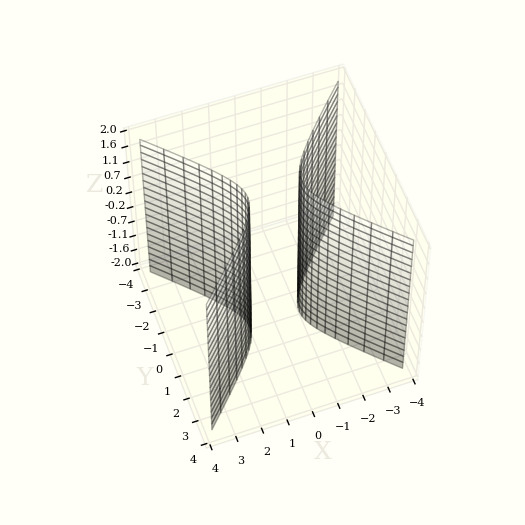
\includegraphics[scale=0.25]{./pics/shkarlupa.png}
        \caption[r]{Гиперболический циллиндр \\ \boxedeq{eq:*}{\frac{x^2}{a^2} - \frac{y^2}{b^2} = \pm1}}
    \end{subfigure}
    ~
  \begin{subfigure}{.25\textwidth}
        \centering
        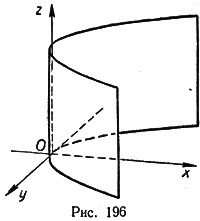
\includegraphics[scale=0.25]{./pics/pip.jpg}
        \caption[r]{Параболический циллиндр \\ \boxedeq{eq:*}{x^2 = \pm 2py}}
    \end{subfigure}
    ~
    \begin{subfigure}{.25\textwidth}
        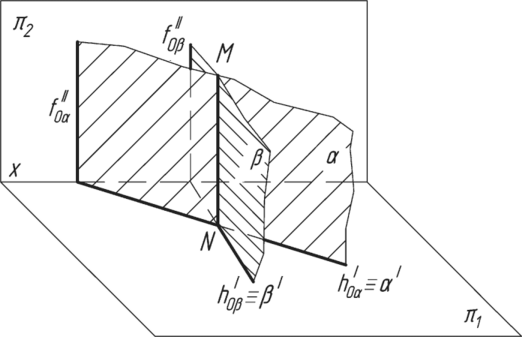
\includegraphics[scale=0.25]{./pics/jizz.png}
        \caption[r]{Пара плоскостей \\ \boxedeq{eq:*}{\frac{x^2}{a^2} - \frac{y^2}{b^2} = 0}}
    \end{subfigure}
    ~
    \begin{subfigure}{.25\textwidth}
        \centering
        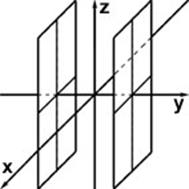
\includegraphics[scale=0.25]{./pics/joq.jpg}
        \caption[r]{Пара плоскостей \\ \boxedeq{eq:*}{\frac{x^2}{a^2} = 1}}
no    \end{subfigure}
\end{figure*}

\chapter{Конические поверхности\\}

Пусть в пространстве зафиксирована точка $A$ и линия $\gamma$. Конической поверхностью с центром в $A$ называется множество точек, лежащих на всех прямых, проходящих
через $A$ и некоторую точку $\in \gamma$. Выберем в пространстве ПСК $Oxyz$  так, чтобы начало координат было центром данной К.П. Тогда этоу К.П. можно задать так:
\par Рассмотрим плоскость $z = 1$, в этой плоскости рассмотрим $\gamma$, заданную уравнением $f(x, y) = 0$ и рассмотрим все прямые, прохрдящие через начало
координат и точку, принадлежащую $\gamma$. Относительно прямых,  проходящих через $O$: если $M(x, y, z) \neq O$ принадлежит такой прямой, $\forall t \in \mathbb{R}: M_t(t_x; t_y; t_z) \in$ этой прямой\footnote{Господа редакторы, что?}.
\par Пусть К.П. $K$ имеет центром $O(0,0,0)$ и определена линией $\gamma$, заданной уравнением $f(x, y) = 0$, тогда рассматривая произвольную точку $M(x; y; z): M \in K \Leftrightarrow \exists t: M_t(t_x; t_y; t_z) \in \gamma \Leftrightarrow \exists t: f(x_t, y_t) = 0 \Leftrightarrow \exists t = \frac{1}{z}: f(\frac{x}{z}, \frac{y}{z}) = 0 \Rightarrow f(\frac{x}{z}, \frac{y}{z})$ - уравнение К.П. $K \setminus \{0\}$.    

\begin{figure*}
        \centering
        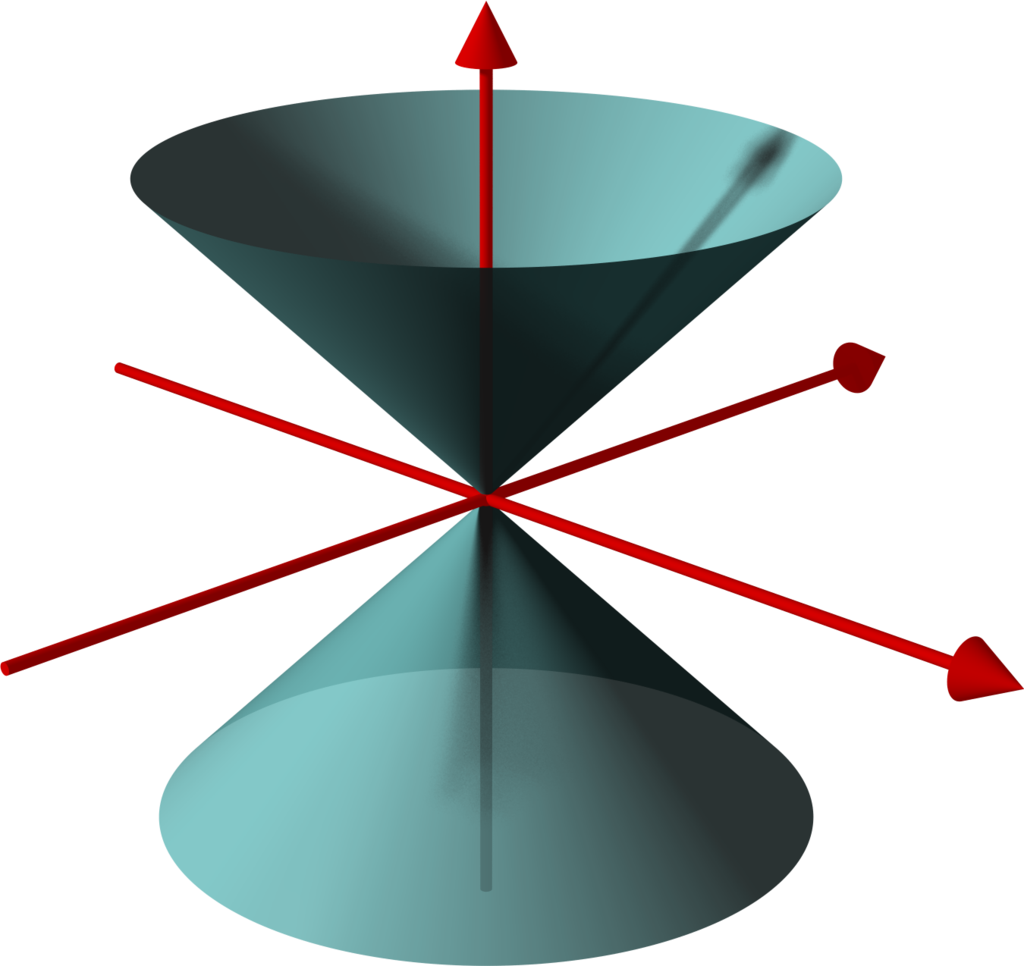
\includegraphics[scale=0.05]{./pics/jiji.png}
[l]{Эллиптический конус \\ \boxedeq{eq:*}{\frac{x^2}{a^2} + \frac{y^2}{b^2} - z^2 = 0}}
\end{figure*} \\

Рассмотрим сечения конуса вращения различными плоскостями. 3 случая, если через начало координат:
\begin{enumerate}
\item Сечение К.В. есть точка $O$
\item Сечение К.В. есть касательная прямая
\item Пара пересекающихся прямых (в начале координат)
\end{enumerate}

Рассмотрим плоскости, не проходящие через начало координат:
\begin{enumerate}
\item Плоскость $\perp Ox$ - окружность.
\item Эллипс(при небольшом угле наклона секущей плоскости).
\item Параболаб если секущая плоскость параллельна одной из образующих.
\item Гипербола, если угол наклона велик.
\end{enumerate}

\chapter{Эллипсоид, Параболоиды, Гиперболоиды\\}

\section{Эллипсоид}

Пусть задана ПСК $Oxyz$. Эллипсоидом называется фигура
\boxedeq{eq:*}{\frac{x^2}{a^2} + \frac{y^2}{b^2} + \frac{z^2}{c^2} = 1}

Все переменные в чётных степенях: Симметричнсть относительно каждой координатной плоскости, оси, начала координат.
Он лежит в коробке размерами $2a \times 2b \times 2c$ ака Дыня в коробке.
Выведем через метод сечений: Режем плоскостями $z = h$, тогда проекция на $Oxy$:
\begin{equation}
  \frac{x^2}{a^2} + \frac{y^2}{b^2} = 1 - \frac{h^2}{c^2}
\end{equation}
3 случая:
\begin{enumerate}

\item $ |h| > c \Leftrightarrow 1 - \frac{h^2}{c^2} < 0 \Rightarrow$ нет таких точек
\item $ |h| = c \Leftrightarrow \frac{x^2}{a^2} + \frac{y^2}{b^2} = 0 \Rightarrow \begin{cases} x = 0 \\ y = 0 \\ z = \pm h = \pm c \end{cases} $
\item $ |h| < c \Leftrightarrow \frac{x^2}{a^2} + \frac{y^2}{b^2}  = 1 - \frac{h^2}{c^2},  \frac{h^2}{c^2} < 1 \Rightarrow  $ Эллипс
  
\end{enumerate}

Аналогичные результаты получим при резании и другими плоскостями. Вершины эллипсоида: $(a; 0; 0), (-a; 0; 0), (0;b;0), \\ (0;-b;0), (0;0;c), (0;0;-c)$, центр эллипсоида: $(0;0;0)$

\section{Гиперболоиды}

\subsection{Однополостные}

\boxedeq{eq:*}{\frac{x^2}{a^2} + \frac{y^2}{b^2} - \frac{z^2}{c^2} = 1} \\ симметриность как у гиперболоида.

Выведем через сечения:
\begin{enumerate}
\item $ z = h: \frac{x^2}{a^2} + \frac{y^2}{b^2} = 1 + \frac{h^2}{a^2}, 1 + \frac{h^2}{a^2} > 0 \Rightarrow \forall h $ эллипс, он растёт, при $h = 0$ горловой эллипс, он самый мелкий.
\item $x = h: \frac{y^2}{b^2} - \frac{z^2}{c^2} = 1 - \frac{h^2}{a^2}:$ \begin{enumerate}
    \item $|h| < a, 1 - \frac{h^2}{a^2} > 0 \Rightarrow $ Гипербола
    \item $|h| = a, \frac{y^2}{b^2} - \frac{z^2}{c^2} = 0 \Rightarrow $ Пара пересекающихся прямых
    \item $|h| > a, 1 - \frac{h^2}{a^2} < 0 \Rightarrow $ Перевёрнутая начальная парабола (свопнуты действительная и мнимая оси)
  \end{enumerate}
\item $y = h$ см. $x = h$
\end{enumerate}

\section{Двуполостный гиперболоид, виброчаша}

\boxedeq{eq:*}{\frac{x^2}{a^2} + \frac{y^2}{b^2} - \frac{z^2}{c^2} = -1} \\ симметричность, как у остальных посонов \\
сечём $z = h$
\begin{equation}
\frac{x^2}{a^2} + \frac{y^2}{b^2} = \frac{h^2}{c^2} - 1
\end{equation}
\begin{enumerate}

\item $|h| < c: \frac{x^2}{a^2} + \frac{y^2}{b^2} = \frac{h^2}{c^2} - 1 \Rightarrow \emptyset$
\item $|h| = c: \frac{x^2}{a^2} + \frac{y^2}{b^2} = 0 \Rightarrow $ Точки, низ и верх виброчаш
  \item $|h| > c: \frac{h^2}{c^2} - 1 > 0 \Rightarrow $ Эллипс
  
\end{enumerate}
теперь сечём $x = h$
  \begin{equation}
    \frac{y^2}{b^2} - \frac{z^2}{c^2} = -1 - \frac{h^2}{a^2} \Rightarrow
  \end{equation}
  Гипербола

\section{Параболоиды}
\subsection{Эллиптический}
\boxedeq{eq:*}{\frac{x^2}{a^2} + \frac{y^2}{b^2} = 2z}
симметричен, но не как виброчаша, его нет сверху, он яма.
сечём $z = h$:
\begin{enumerate}
\item $h < 0: \frac{x^2}{a^2} + \frac{y^2}{b^2} < 0 \Rightarrow \emptyset$
\item $h = 0: \frac{x^2}{a^2} + \frac{y^2}{b^2} = 0 \Rightarrow (0;0;0)$
\item $h > 0: \frac{x^2}{a^2} + \frac{y^2}{b^2} = 2h \Rightarrow $ Эллипс
\end{enumerate}
теперь режем $x=h$ (также будет и с $y = h$)
\begin{equation}
  \frac{h^2}{a^2} + \frac{y^2}{b^2} = 2z \Leftrightarrow \frac{y^2}{b^2} = 2(z - \frac{h^2}{2a^2})
\end{equation}
получаем сдвигающуюсю вверх на $\frac{h^2}{2b^2}$ параболу.
\subsection{Гиперболический Параболоил ака Седло для коня из коничесикх поверхноствей}
\boxedeq{eq:*}{\frac{x^2}{a^2} - \frac{y^2}{b^2} = 2z}
Чёткий, симметричный, но не относительно $Oxy, O$
Режем $z = h$
\begin{enumerate}
\item $h < 0: \frac{x^2}{a^2} - \frac{y^2}{b^2} < 0 \Rightarrow $ Гипербола(действительная $Oy$)
\item $h = 0: \frac{x^2}{a^2} - \frac{y^2}{b^2} = 0 \Rightarrow $ 2 пересекающиеся прямвые
  \item $h > 0: \frac{x^2}{a^2} - \frac{y^2}{b^2} = 2h \Rightarrow $ Гипербола(действительная $Ox$)
Теперь $x = h$
\begin{equation}
  \frac{h^2}{a^2} - \frac{y^2}{b^2} = 2z \Rightarrow \frac{-y^2}{b^2} = 2(z - \frac{h^2}{a^2})
\end{equation}
это парабола, полученная сдвигом на $\frac{h^2}{2a^2}$
Теперь $y = h$
\begin{equation}
  \frac{x^2}{a^2} = 2(z + \frac{h^2}{b^2})
\end{equation}
Это парабола, сдвигающаяся вниз

\end{document}
